\documentclass[11pt,compress,t,notes=noshow, aspectratio=169, xcolor=table]{beamer}
% deactivate beamer navigation
%\setbeamertemplate{navigation symbols}{}
%\usepackage{geometry}
%\geometry{papersize={180mm, 135mm}, top=-1.5mm} % 210mm, 297mm

% set path of iml lecture here, e.g., relative to the current dir
\newcommand{\pathiml}{../../slides/03_feature-effects/}
\usepackage{../../style/lmu-lecture}

% Defines macros and environments
\usepackage[]{graphicx}
\usepackage[]{color}
% maxwidth is the original width if it is less than linewidth
% otherwise use linewidth (to make sure the graphics do not exceed the margin)
\makeatletter
\def\maxwidth{ %
\ifdim\Gin@nat@width>\linewidth
\linewidth
\else
\Gin@nat@width
\fi
}
\makeatother
%\usepackage[fontsize=10.5pt]{scrextend}
\definecolor{ggred}{rgb}{0.973, 0.463, 0.427}
\definecolor{ggblue}{rgb}{0, 0.749, 0.769}
\definecolor{fgcolor}{rgb}{0.345, 0.345, 0.345}
\newcommand{\hlnum}[1]{\textcolor[rgb]{0.686,0.059,0.569}{#1}}%
\newcommand{\hlstr}[1]{\textcolor[rgb]{0.192,0.494,0.8}{#1}}%
\newcommand{\hlcom}[1]{\textcolor[rgb]{0.678,0.584,0.686}{\textit{#1}}}%
\newcommand{\hlopt}[1]{\textcolor[rgb]{0,0,0}{#1}}%
\newcommand{\hlstd}[1]{\textcolor[rgb]{0.345,0.345,0.345}{#1}}%
\newcommand{\hlkwa}[1]{\textcolor[rgb]{0.161,0.373,0.58}{\textbf{#1}}}%
\newcommand{\hlkwb}[1]{\textcolor[rgb]{0.69,0.353,0.396}{#1}}%
\newcommand{\hlkwc}[1]{\textcolor[rgb]{0.333,0.667,0.333}{#1}}%
\newcommand{\hlkwd}[1]{\textcolor[rgb]{0.737,0.353,0.396}{\textbf{#1}}}%
\newcommand{\predvar}{Var\left[\hat{f}(\xv)\right]}
\let\hlipl\hlkwb

\usepackage{pdfpages}
\usepackage{framed}
\makeatletter
\newenvironment{kframe}{%
\def\at@end@of@kframe{}%
\ifinner\ifhmode%
\def\at@end@of@kframe{\end{minipage}}%
\begin{minipage}{\columnwidth}%
\fi\fi%
\def\FrameCommand##1{\hskip\@totalleftmargin \hskip-\fboxsep
\colorbox{shadecolor}{##1}\hskip-\fboxsep
% There is no \\@totalrightmargin, so:
\hskip-\linewidth \hskip-\@totalleftmargin \hskip\columnwidth}%
\MakeFramed {\advance\hsize-\width
\@totalleftmargin\z@ \linewidth\hsize
\@setminipage}}%
{\par\unskip\endMakeFramed%
\at@end@of@kframe}
\makeatother

\definecolor{shadecolor}{rgb}{.97, .97, .97}
\definecolor{messagecolor}{rgb}{0, 0, 0}
\definecolor{warningcolor}{rgb}{1, 0, 1}
\definecolor{errorcolor}{rgb}{1, 0, 0}
\newenvironment{knitrout}{}{} % an empty environment to be redefined in TeX

\usepackage{alltt}
\newcommand{\SweaveOpts}[1]{}  % do not interfere with LaTeX
\newcommand{\SweaveInput}[1]{} % because they are not real TeX commands
\newcommand{\Sexpr}[1]{}       % will only be parsed by R

\usepackage[english]{babel}
\usepackage[utf8]{inputenc}

\usepackage[export]{adjustbox}
\usepackage{dsfont}
\usepackage{verbatim}
\usepackage{amsmath}
\usepackage{amsfonts}
\usepackage{bm}
\usepackage{csquotes}
\usepackage{multirow}
\usepackage{longtable}
\usepackage{booktabs}
\usepackage{enumerate}
\usepackage[absolute,overlay]{textpos}
\usepackage{psfrag}
\usepackage{algorithm}
\usepackage{algpseudocode}
\usepackage{eqnarray}
\usepackage{arydshln}
\usepackage{tabularx}
\usepackage{placeins}
\usepackage{tikz}
\usepackage{setspace}
\usepackage{colortbl}
\usepackage{mathtools}
\usepackage{wrapfig}
\usepackage{bm}
\usepackage[backend=biber]{biblatex}

\usetikzlibrary{tikzmark, shapes,arrows,automata,positioning,calc,chains,trees,  shadows, decorations.pathreplacing}
\tikzset{
%Define standard arrow tip
>=stealth',
%Define style for boxes
punkt/.style={
rectangle,
rounded corners,
draw=black, very thick,
text width=6.5em,
minimum height=2em,
text centered},
% Define arrow style
pil/.style={
->,
thick,
shorten <=2pt,
shorten >=2pt,}
}

\usepackage{subfig}

\usepackage{bbm}
%\newcommand\hmmax{0}
%\newcommand\bmmax{0}
% basic latex stuff
\newcommand{\pkg}[1]{{\fontseries{b}\selectfont #1}} %fontstyle for R packages
\newcommand{\lz}{\vspace{0.5cm}} %vertical space
\newcommand{\dlz}{\vspace{1cm}} %double vertical space
\newcommand{\oneliner}[1] % Oneliner for important statements
{\begin{block}{}\begin{center}\begin{Large}#1\end{Large}\end{center}\end{block}}

% Latexmath Notation
% math spaces
\ifdefined\N                                                                
\renewcommand{\N}{\mathds{N}} % N, naturals
\else \newcommand{\N}{\mathds{N}} \fi 
\newcommand{\Z}{\mathds{Z}} % Z, integers
\newcommand{\Q}{\mathds{Q}} % Q, rationals
\newcommand{\R}{\mathds{R}} % R, reals
\ifdefined\C 
  \renewcommand{\C}{\mathds{C}} % C, complex
\else \newcommand{\C}{\mathds{C}} \fi
\newcommand{\continuous}{\mathcal{C}} % C, space of continuous functions
\newcommand{\M}{\mathcal{M}} % machine numbers
\newcommand{\epsm}{\epsilon_m} % maximum error

% counting / finite sets
\newcommand{\setzo}{\{0, 1\}} % set 0, 1
\newcommand{\setmp}{\{-1, +1\}} % set -1, 1
\newcommand{\unitint}{[0, 1]} % unit interval

% basic math stuff
\newcommand{\xt}{\tilde x} % x tilde
\newcommand{\argmax}{\operatorname{arg\,max}} % argmax
\newcommand{\argmin}{\operatorname{arg\,min}} % argmin
\newcommand{\argminlim}{\mathop{\mathrm{arg\,min}}\limits} % argmax with limits
\newcommand{\argmaxlim}{\mathop{\mathrm{arg\,max}}\limits} % argmin with limits  
\newcommand{\sign}{\operatorname{sign}} % sign, signum
\newcommand{\I}{\mathbb{I}} % I, indicator
\newcommand{\order}{\mathcal{O}} % O, order
\newcommand{\pd}[2]{\frac{\partial{#1}}{\partial #2}} % partial derivative
\newcommand{\floorlr}[1]{\left\lfloor #1 \right\rfloor} % floor
\newcommand{\ceillr}[1]{\left\lceil #1 \right\rceil} % ceiling

% sums and products
\newcommand{\sumin}{\sum\limits_{i=1}^n} % summation from i=1 to n
\newcommand{\sumim}{\sum\limits_{i=1}^m} % summation from i=1 to m
\newcommand{\sumjn}{\sum\limits_{j=1}^n} % summation from j=1 to p
\newcommand{\sumjp}{\sum\limits_{j=1}^p} % summation from j=1 to p
\newcommand{\sumik}{\sum\limits_{i=1}^k} % summation from i=1 to k
\newcommand{\sumkg}{\sum\limits_{k=1}^g} % summation from k=1 to g
\newcommand{\sumjg}{\sum\limits_{j=1}^g} % summation from j=1 to g
\newcommand{\meanin}{\frac{1}{n} \sum\limits_{i=1}^n} % mean from i=1 to n
\newcommand{\meanim}{\frac{1}{m} \sum\limits_{i=1}^m} % mean from i=1 to n
\newcommand{\meankg}{\frac{1}{g} \sum\limits_{k=1}^g} % mean from k=1 to g
\newcommand{\prodin}{\prod\limits_{i=1}^n} % product from i=1 to n
\newcommand{\prodkg}{\prod\limits_{k=1}^g} % product from k=1 to g
\newcommand{\prodjp}{\prod\limits_{j=1}^p} % product from j=1 to p

% linear algebra
\newcommand{\one}{\boldsymbol{1}} % 1, unitvector
\newcommand{\zero}{\mathbf{0}} % 0-vector
\newcommand{\id}{\boldsymbol{I}} % I, identity
\newcommand{\diag}{\operatorname{diag}} % diag, diagonal
\newcommand{\trace}{\operatorname{tr}} % tr, trace
\newcommand{\spn}{\operatorname{span}} % span
\newcommand{\scp}[2]{\left\langle #1, #2 \right\rangle} % <.,.>, scalarproduct
\newcommand{\mat}[1]{\begin{pmatrix} #1 \end{pmatrix}} % short pmatrix command
\newcommand{\Amat}{\mathbf{A}} % matrix A
\newcommand{\Deltab}{\mathbf{\Delta}} % error term for vectors

% basic probability + stats
\renewcommand{\P}{\mathds{P}} % P, probability
\newcommand{\E}{\mathds{E}} % E, expectation
\newcommand{\var}{\mathsf{Var}} % Var, variance
\newcommand{\cov}{\mathsf{Cov}} % Cov, covariance
\newcommand{\corr}{\mathsf{Corr}} % Corr, correlation
\newcommand{\normal}{\mathcal{N}} % N of the normal distribution
\newcommand{\iid}{\overset{i.i.d}{\sim}} % dist with i.i.d superscript
\newcommand{\distas}[1]{\overset{#1}{\sim}} % ... is distributed as ...

% machine learning
\newcommand{\Xspace}{\mathcal{X}} % X, input space
\newcommand{\Yspace}{\mathcal{Y}} % Y, output space
\newcommand{\nset}{\{1, \ldots, n\}} % set from 1 to n
\newcommand{\pset}{\{1, \ldots, p\}} % set from 1 to p
\newcommand{\gset}{\{1, \ldots, g\}} % set from 1 to g
\newcommand{\Pxy}{\mathbb{P}_{xy}} % P_xy
\newcommand{\Exy}{\mathbb{E}_{xy}} % E_xy: Expectation over random variables xy
\newcommand{\xv}{\mathbf{x}} % vector x (bold)
\newcommand{\xtil}{\tilde{\mathbf{x}}} % vector x-tilde (bold)
\newcommand{\yv}{\mathbf{y}} % vector y (bold)
\newcommand{\xy}{(\xv, y)} % observation (x, y)
\newcommand{\xvec}{\left(x_1, \ldots, x_p\right)^\top} % (x1, ..., xp) 
\newcommand{\Xmat}{\mathbf{X}} % Design matrix
\newcommand{\allDatasets}{\mathds{D}} % The set of all datasets
\newcommand{\allDatasetsn}{\mathds{D}_n}  % The set of all datasets of size n 
\newcommand{\D}{\mathcal{D}} % D, data
\newcommand{\Dn}{\D_n} % D_n, data of size n
\newcommand{\Dtrain}{\mathcal{D}_{\text{train}}} % D_train, training set
\newcommand{\Dtest}{\mathcal{D}_{\text{test}}} % D_test, test set
\newcommand{\xyi}[1][i]{\left(\xv^{(#1)}, y^{(#1)}\right)} % (x^i, y^i), i-th observation
\newcommand{\Dset}{\left( \xyi[1], \ldots, \xyi[n]\right)} % {(x1,y1)), ..., (xn,yn)}, data
\newcommand{\defAllDatasetsn}{(\Xspace \times \Yspace)^n} % Def. of the set of all datasets of size n 
\newcommand{\defAllDatasets}{\bigcup_{n \in \N}(\Xspace \times \Yspace)^n} % Def. of the set of all datasets 
\newcommand{\xdat}{\left\{ \xv^{(1)}, \ldots, \xv^{(n)}\right\}} % {x1, ..., xn}, input data
\newcommand{\ydat}{\left\{ \yv^{(1)}, \ldots, \yv^{(n)}\right\}} % {y1, ..., yn}, input data
\newcommand{\yvec}{\left(y^{(1)}, \hdots, y^{(n)}\right)^\top} % (y1, ..., yn), vector of outcomes
\renewcommand{\xi}[1][i]{\xv^{(#1)}} % x^i, i-th observed value of x
\newcommand{\yi}[1][i]{y^{(#1)}} % y^i, i-th observed value of y 
\newcommand{\xivec}{\left(x^{(i)}_1, \ldots, x^{(i)}_p\right)^\top} % (x1^i, ..., xp^i), i-th observation vector
\newcommand{\xj}{\xv_j} % x_j, j-th feature
\newcommand{\xjvec}{\left(x^{(1)}_j, \ldots, x^{(n)}_j\right)^\top} % (x^1_j, ..., x^n_j), j-th feature vector
\newcommand{\phiv}{\mathbf{\phi}} % Basis transformation function phi
\newcommand{\phixi}{\mathbf{\phi}^{(i)}} % Basis transformation of xi: phi^i := phi(xi)

%%%%%% ml - models general
\newcommand{\lamv}{\bm{\lambda}} % lambda vector, hyperconfiguration vector
\newcommand{\Lam}{\bm{\Lambda}}	 % Lambda, space of all hpos
% Inducer / Inducing algorithm
\newcommand{\preimageInducer}{\left(\defAllDatasets\right)\times\Lam} % Set of all datasets times the hyperparameter space
\newcommand{\preimageInducerShort}{\allDatasets\times\Lam} % Set of all datasets times the hyperparameter space
% Inducer / Inducing algorithm
\newcommand{\ind}{\mathcal{I}} % Inducer, inducing algorithm, learning algorithm 

% continuous prediction function f
\newcommand{\ftrue}{f_{\text{true}}}  % True underlying function (if a statistical model is assumed)
\newcommand{\ftruex}{\ftrue(\xv)} % True underlying function (if a statistical model is assumed)
\newcommand{\fx}{f(\xv)} % f(x), continuous prediction function
\newcommand{\fdomains}{f: \Xspace \rightarrow \R^g} % f with domain and co-domain
\newcommand{\Hspace}{\mathcal{H}} % hypothesis space where f is from
\newcommand{\fbayes}{f^{\ast}} % Bayes-optimal model
\newcommand{\fxbayes}{f^{\ast}(\xv)} % Bayes-optimal model
\newcommand{\fkx}[1][k]{f_{#1}(\xv)} % f_j(x), discriminant component function
\newcommand{\fh}{\hat{f}} % f hat, estimated prediction function
\newcommand{\fxh}{\fh(\xv)} % fhat(x)
\newcommand{\fxt}{f(\xv ~|~ \thetab)} % f(x | theta)
\newcommand{\fxi}{f\left(\xv^{(i)}\right)} % f(x^(i))
\newcommand{\fxih}{\hat{f}\left(\xv^{(i)}\right)} % f(x^(i))
\newcommand{\fxit}{f\left(\xv^{(i)} ~|~ \thetab\right)} % f(x^(i) | theta)
\newcommand{\fhD}{\fh_{\D}} % fhat_D, estimate of f based on D
\newcommand{\fhDtrain}{\fh_{\Dtrain}} % fhat_Dtrain, estimate of f based on D
\newcommand{\fhDnlam}{\fh_{\Dn, \lamv}} %model learned on Dn with hp lambda
\newcommand{\fhDlam}{\fh_{\D, \lamv}} %model learned on D with hp lambda
\newcommand{\fhDnlams}{\fh_{\Dn, \lamv^\ast}} %model learned on Dn with optimal hp lambda 
\newcommand{\fhDlams}{\fh_{\D, \lamv^\ast}} %model learned on D with optimal hp lambda 

% discrete prediction function h
\newcommand{\hx}{h(\xv)} % h(x), discrete prediction function
\newcommand{\hh}{\hat{h}} % h hat
\newcommand{\hxh}{\hat{h}(\xv)} % hhat(x)
\newcommand{\hxt}{h(\xv | \thetab)} % h(x | theta)
\newcommand{\hxi}{h\left(\xi\right)} % h(x^(i))
\newcommand{\hxit}{h\left(\xi ~|~ \thetab\right)} % h(x^(i) | theta)
\newcommand{\hbayes}{h^{\ast}} % Bayes-optimal classification model
\newcommand{\hxbayes}{h^{\ast}(\xv)} % Bayes-optimal classification model

% yhat
\newcommand{\yh}{\hat{y}} % yhat for prediction of target
\newcommand{\yih}{\hat{y}^{(i)}} % yhat^(i) for prediction of ith targiet
\newcommand{\resi}{\yi- \yih}

% theta
\newcommand{\thetah}{\hat{\theta}} % theta hat
\newcommand{\thetab}{\bm{\theta}} % theta vector
\newcommand{\thetabh}{\bm{\hat\theta}} % theta vector hat
\newcommand{\thetat}[1][t]{\thetab^{[#1]}} % theta^[t] in optimization
\newcommand{\thetatn}[1][t]{\thetab^{[#1 +1]}} % theta^[t+1] in optimization
\newcommand{\thetahDnlam}{\thetabh_{\Dn, \lamv}} %theta learned on Dn with hp lambda
\newcommand{\thetahDlam}{\thetabh_{\D, \lamv}} %theta learned on D with hp lambda
\newcommand{\mint}{\min_{\thetab \in \Theta}} % min problem theta
\newcommand{\argmint}{\argmin_{\thetab \in \Theta}} % argmin theta

% densities + probabilities
% pdf of x 
\newcommand{\pdf}{p} % p
\newcommand{\pdfx}{p(\xv)} % p(x)
\newcommand{\pixt}{\pi(\xv~|~ \thetab)} % pi(x|theta), pdf of x given theta
\newcommand{\pixit}[1][i]{\pi\left(\xi[#1] ~|~ \thetab\right)} % pi(x^i|theta), pdf of x given theta
\newcommand{\pixii}[1][i]{\pi\left(\xi[#1]\right)} % pi(x^i), pdf of i-th x 

% pdf of (x, y)
\newcommand{\pdfxy}{p(\xv,y)} % p(x, y)
\newcommand{\pdfxyt}{p(\xv, y ~|~ \thetab)} % p(x, y | theta)
\newcommand{\pdfxyit}{p\left(\xi, \yi ~|~ \thetab\right)} % p(x^(i), y^(i) | theta)

% pdf of x given y
\newcommand{\pdfxyk}[1][k]{p(\xv | y= #1)} % p(x | y = k)
\newcommand{\lpdfxyk}[1][k]{\log p(\xv | y= #1)} % log p(x | y = k)
\newcommand{\pdfxiyk}[1][k]{p\left(\xi | y= #1 \right)} % p(x^i | y = k)

% prior probabilities
\newcommand{\pik}[1][k]{\pi_{#1}} % pi_k, prior
\newcommand{\lpik}[1][k]{\log \pi_{#1}} % log pi_k, log of the prior
\newcommand{\pit}{\pi(\thetab)} % Prior probability of parameter theta

% posterior probabilities
\newcommand{\post}{\P(y = 1 ~|~ \xv)} % P(y = 1 | x), post. prob for y=1
\newcommand{\postk}[1][k]{\P(y = #1 ~|~ \xv)} % P(y = k | y), post. prob for y=k
\newcommand{\pidomains}{\pi: \Xspace \rightarrow \unitint} % pi with domain and co-domain
\newcommand{\pibayes}{\pi^{\ast}} % Bayes-optimal classification model
\newcommand{\pixbayes}{\pi^{\ast}(\xv)} % Bayes-optimal classification model
\newcommand{\pix}{\pi(\xv)} % pi(x), P(y = 1 | x)
\newcommand{\piv}{\bm{\pi}} % pi, bold, as vector
\newcommand{\pikx}[1][k]{\pi_{#1}(\xv)} % pi_k(x), P(y = k | x)
\newcommand{\pikxt}[1][k]{\pi_{#1}(\xv ~|~ \thetab)} % pi_k(x | theta), P(y = k | x, theta)
\newcommand{\pixh}{\hat \pi(\xv)} % pi(x) hat, P(y = 1 | x) hat
\newcommand{\pikxh}[1][k]{\hat \pi_{#1}(\xv)} % pi_k(x) hat, P(y = k | x) hat
\newcommand{\pixih}{\hat \pi(\xi)} % pi(x^(i)) with hat
\newcommand{\pikxih}[1][k]{\hat \pi_{#1}(\xi)} % pi_k(x^(i)) with hat
\newcommand{\pdfygxt}{p(y ~|~\xv, \thetab)} % p(y | x, theta)
\newcommand{\pdfyigxit}{p\left(\yi ~|~\xi, \thetab\right)} % p(y^i |x^i, theta)
\newcommand{\lpdfygxt}{\log \pdfygxt } % log p(y | x, theta)
\newcommand{\lpdfyigxit}{\log \pdfyigxit} % log p(y^i |x^i, theta)

% probababilistic
\newcommand{\bayesrulek}[1][k]{\frac{\P(\xv | y= #1) \P(y= #1)}{\P(\xv)}} % Bayes rule
\newcommand{\muk}{\bm{\mu_k}} % mean vector of class-k Gaussian (discr analysis) 

% residual and margin
\newcommand{\eps}{\epsilon} % residual, stochastic
\newcommand{\epsi}{\epsilon^{(i)}} % epsilon^i, residual, stochastic
\newcommand{\epsh}{\hat{\epsilon}} % residual, estimated
\newcommand{\yf}{y \fx} % y f(x), margin
\newcommand{\yfi}{\yi \fxi} % y^i f(x^i), margin
\newcommand{\Sigmah}{\hat \Sigma} % estimated covariance matrix
\newcommand{\Sigmahj}{\hat \Sigma_j} % estimated covariance matrix for the j-th class

% ml - loss, risk, likelihood
\newcommand{\Lyf}{L\left(y, f\right)} % L(y, f), loss function
\newcommand{\Lypi}{L\left(y, \pi\right)} % L(y, pi), loss function
\newcommand{\Lxy}{L\left(y, \fx\right)} % L(y, f(x)), loss function
\newcommand{\Lxyi}{L\left(\yi, \fxi\right)} % loss of observation
\newcommand{\Lxyt}{L\left(y, \fxt\right)} % loss with f parameterized
\newcommand{\Lxyit}{L\left(\yi, \fxit\right)} % loss of observation with f parameterized
\newcommand{\Lxym}{L\left(\yi, f\left(\bm{\tilde{x}}^{(i)} ~|~ \thetab\right)\right)} % loss of observation with f parameterized
\newcommand{\Lpixy}{L\left(y, \pix\right)} % loss in classification
\newcommand{\Lpiv}{L\left(y, \piv\right)} % loss in classification
\newcommand{\Lpixyi}{L\left(\yi, \pixii\right)} % loss of observation in classification
\newcommand{\Lpixyt}{L\left(y, \pixt\right)} % loss with pi parameterized
\newcommand{\Lpixyit}{L\left(\yi, \pixit\right)} % loss of observation with pi parameterized
\newcommand{\Lhxy}{L\left(y, \hx\right)} % L(y, h(x)), loss function on discrete classes
\newcommand{\Lr}{L\left(r\right)} % L(r), loss defined on residual (reg) / margin (classif)
\newcommand{\lone}{|y - \fx|} % L1 loss
\newcommand{\ltwo}{\left(y - \fx\right)^2} % L2 loss
\newcommand{\lbernoullimp}{\ln(1 + \exp(-y \cdot \fx))} % Bernoulli loss for -1, +1 encoding
\newcommand{\lbernoullizo}{- y \cdot \fx + \log(1 + \exp(\fx))} % Bernoulli loss for 0, 1 encoding
\newcommand{\lcrossent}{- y \log \left(\pix\right) - (1 - y) \log \left(1 - \pix\right)} % cross-entropy loss
\newcommand{\lbrier}{\left(\pix - y \right)^2} % Brier score
\newcommand{\risk}{\mathcal{R}} % R, risk
\newcommand{\riskbayes}{\mathcal{R}^\ast}
\newcommand{\riskf}{\risk(f)} % R(f), risk
\newcommand{\riskdef}{\E_{y|\xv}\left(\Lxy \right)} % risk def (expected loss)
\newcommand{\riskt}{\mathcal{R}(\thetab)} % R(theta), risk
\newcommand{\riske}{\mathcal{R}_{\text{emp}}} % R_emp, empirical risk w/o factor 1 / n
\newcommand{\riskeb}{\bar{\mathcal{R}}_{\text{emp}}} % R_emp, empirical risk w/ factor 1 / n
\newcommand{\riskef}{\riske(f)} % R_emp(f)
\newcommand{\risket}{\mathcal{R}_{\text{emp}}(\thetab)} % R_emp(theta)
\newcommand{\riskr}{\mathcal{R}_{\text{reg}}} % R_reg, regularized risk
\newcommand{\riskrt}{\mathcal{R}_{\text{reg}}(\thetab)} % R_reg(theta)
\newcommand{\riskrf}{\riskr(f)} % R_reg(f)
\newcommand{\riskrth}{\hat{\mathcal{R}}_{\text{reg}}(\thetab)} % hat R_reg(theta)
\newcommand{\risketh}{\hat{\mathcal{R}}_{\text{emp}}(\thetab)} % hat R_emp(theta)
\newcommand{\LL}{\mathcal{L}} % L, likelihood
\newcommand{\LLt}{\mathcal{L}(\thetab)} % L(theta), likelihood
\newcommand{\LLtx}{\mathcal{L}(\thetab | \xv)} % L(theta|x), likelihood
\newcommand{\logl}{\ell} % l, log-likelihood
\newcommand{\loglt}{\logl(\thetab)} % l(theta), log-likelihood
\newcommand{\logltx}{\logl(\thetab | \xv)} % l(theta|x), log-likelihood
\newcommand{\errtrain}{\text{err}_{\text{train}}} % training error
\newcommand{\errtest}{\text{err}_{\text{test}}} % test error
\newcommand{\errexp}{\overline{\text{err}_{\text{test}}}} % avg training error

% lm
\newcommand{\thx}{\thetab^\top \xv} % linear model
\newcommand{\olsest}{(\Xmat^\top \Xmat)^{-1} \Xmat^\top \yv} % OLS estimator in LM 

%%%%%% perturbed data
\usepackage{xifthen}
\newcommand{\pert}[3]{\ifthenelse{\equal{#2}{}}{\tilde{#1}}{\ifthenelse{\equal{#3}{}}{\tilde{#1}^{#2}}{\tilde{#1}^{#2|#3}}}}	% command to express that for #1 the subset #2 was perturbed given subset #3

%%%%%% marginalized functions
\newcommand{\fj}{f_j} % marginal function f_j, depending on feature j
\newcommand{\fnj}{f_{-j}} % marginal function f_{-j}, depending on all features but j
\newcommand{\fS}{f_S} % marginal function f_S depending on feature set S
\newcommand{\fnj}{f_{-S}} % marginal function f_{-S}, depending on all features but features in S
\newcommand{\fC}{f_C} % marginal function f_C depending on feature set C
\newcommand{\fhj}{\fh_j} % marginal function fh_j, depending on feature j
\newcommand{\fhnj}{\fh_{-j}} % marginal function fh_{-j}, depending on all features but j
\newcommand{\fhS}{\fh_S} % marginal function fh_S depending on feature set S
\newcommand{\fhnS}{\fh_{-S}} % marginal function fh_{-S}, depending on all features but features in S
\newcommand{\fhC}{\fh_C} % marginal function fh_C depending on feature set C
\newcommand{\XSmat}{\Xmat_S} % Design matrix subset
\newcommand{\XnSmat}{\Xmat__{-S}} % Design matrix subset without S
\newcommand{\XCmat}{\Xmat_C} % Design matrix subset
\newcommand{\Xnj}{\Xmat_{-j}} % Design matrix subset -j = {1, .., j-1, j+1, ..., p}

%%%%% Shapley values
\newcommand{\Scupj}{S \cup \{j\}} % coalition S but without player j
\newcommand{\Scupk}{S \cup \{k\}} % coalition S but without player k
\newcommand{\SsubP}{S \subseteq P} % coalition S subset of P
\newcommand{\SsubPnoj}{\SsubP \setminus \{j\}} % coalition S subset of P without player j
\newcommand{\SsubPnojk}{\SsubP \setminus \{j,k\}} % coalition S subset of P without player k
\newcommand{\phiij}{\hat{\phi}_j^{(i)}} % Shapley value for feature j and observation i

%%%%% LIME 
\newcommand{\Gspace}{\mathcal{G}} % Hypothesis space for surrogate model
\newcommand{\neigh}{\phi_{\xv}} % Proximity measure
\newcommand{\zv}{\mathbf{z}} % Sampled datapoints for surrogate
\newcommand{\Zspace}{\mathcal{Z}} % Space of sampled datapoints
\newcommand{\Gower}{d_G} % Gower distance


\newcommand{\indep}{\perp}
\newcommand{\Ind}{\mathcal{I}}

%new environments
\newenvironment{vbframe}  %frame with breaks and verbatim
{
\begin{frame}%[containsverbatim,allowframebreaks]
}
{
\end{frame}
}

% \newenvironment{vframe}  %frame with verbatim without breaks (to avoid numbering one slided frames)
% {
%  \begin{frame}[containsverbatim]
% }
% {
% \end{frame}
% }

\newenvironment{blocki}[1]   % itemize block
{
 \begin{block}{#1}\begin{itemize}
}
{
\end{itemize}\end{block}
}

\newenvironment{fragileframe}[2]{  %fragile frame with framebreaks
\begin{frame}[allowframebreaks, fragile, environment = fragileframe]
\frametitle{#1}
#2}
{\end{frame}}


\newcommand{\myframe}[2]{  %short for frame with framebreaks
\begin{frame}[allowframebreaks]
\frametitle{#1}
#2
\end{frame}}

\newcommand{\remark}[1]{
  \textbf{Remark:} #1
}


\newenvironment{deleteframe}
{
\begingroup
\usebackgroundtemplate{
\includegraphics[width=\paperwidth,height=\paperheight]{../style/color/red.png}}
 \begin{frame}
}
{
\end{frame}
\endgroup
}
\newenvironment{simplifyframe}
{
\begingroup
\usebackgroundtemplate{
\includegraphics[width=\paperwidth,height=\paperheight]{../style/color/yellow.png}}
 \begin{frame}
}
{
\end{frame}
\endgroup
}\newenvironment{draftframe}
{
\begingroup
\usebackgroundtemplate{
\includegraphics[width=\paperwidth,height=\paperheight]{../style/color/green.jpg}}
 \begin{frame}
}
{
\end{frame}
\endgroup
}
% https://tex.stackexchange.com/a/261480: textcolor that works in mathmode
\makeatletter
\renewcommand*{\@textcolor}[3]{%
  \protect\leavevmode
  \begingroup
    \color#1{#2}#3%
  \endgroup
}
\makeatother

% \makeatletter
% %\newcommand\notsotiny{\@setfontsize\notsotiny\@vipt\@viipt}
% \newcommand\notsotiny{\@setfontsize\notsotiny{6.31415}{7.1828}}
% \makeatother

\providecommand{\tightlist}{%
  \setlength{\itemsep}{0pt}\setlength{\parskip}{0pt}}

%\setbeamerfont{footnote}{size=\tiny}
\usepackage[hang,flushmargin]{footmisc}
\renewcommand*{\footnotelayout}{\tiny}
\renewcommand*{\thefootnote}{} %\fnsymbol{footnote}

% https://tex.stackexchange.com/questions/638616/beamer-frametitle-always-uppercase-for-text-but-not-for-href-or-url
\usepackage{textcase}

% https://stackoverflow.com/questions/377301/is-there-a-latex-command-to-make-text-all-lower-caps
%\usepackage[overload]{textcase}
%\setbeamertemplate{frametitle}{\MakeTextUppercase{\insertframetitle}}
%\setbeamertemplate{frametitle}{\expandafter\uppercase\expandafter\insertframetitle}

\setbeamertemplate{frametitle}{\MakeTextUppercase{\insertframetitle}}
\newcommand{\citebutton}[2]{%
\NoCaseChange{\resizebox{!}{9pt}{\protect\beamergotobutton{\href{#2}{#1}}}}%
}

%\setbeamertemplate{frametitle}{\expandafter\uppercase\expandafter\insertframetitle}
%\newcommand{\citebutton}[2]{%
%\href{#2}{\footnotesize\color{black!60}[#1]}
%\resizebox{!}{9pt}{\beamergotobutton{\lowercase{\href{#2}}{#1}}}% \MakeLowercase
%}
%\newcommand{\lit}[2]{\href{#2}{\footnotesize\color{black!60}[#1]}}

\newcommand{\lit}[2]{\href{#2}{\footnotesize\color{black!60}[#1]}}

\let\code=\texttt
\let\proglang=\textsf

\setkeys{Gin}{width=0.9\textwidth}

% https://tex.stackexchange.com/questions/30720/footnote-without-a-marker
% \makeatletter
% \def\blfootnote{\gdef\@thefnmark{}\@footnotetext}
% \makeatother

% https://tex.stackexchange.com/questions/357717/beamer-allowframebreaks-option-and-vertical-spacing-when-using-lists-itemize
% \setbeamertemplate{frametitle continuation}{%
%     (\insertcontinuationcount)%
%     \ifnum\insertcontinuationcount>1%
%     \vspace*{\topsep}%
%     \else%
%     %
%     \fi%
% }


\newcommand\tab[1][1cm]{\hspace*{#1}}
\tikzset{main node/.style={rectangle,draw,minimum size=1cm,inner sep=4pt},}

\usepackage[export]{adjustbox}
\usepackage[most]{tcolorbox}

\newtcolorbox{BlueBox}[2][]{%
   enhanced,
   colback   = blue!5!white,
   colframe  = blue!65!black,
   arc       = 1mm,
   outer arc = 1mm,
   fonttitle = \Large\slshape\textbf,
   center title,
   title     = #2,
   #1}

\title{Interpretable Machine Learning}
% \author{LMU}
%\institute{\href{https://compstat-lmu.github.io/lecture_iml/}{compstat-lmu.github.io/lecture\_iml}}
\date{}


\newcommand{\mysectionslide}{
\begin{frame}[plain]
    %\global\advance\c@lecture by -1
    \vspace*{0.5 cm}
    \LARGE\bfseries\inserttitle
    \vspace*{0.5 cm}

    \ifx\lecturesection\@empty\relax\else%
    {\lecturesection}%
    \fi%

\ifcsname learninggoals\endcsname
  {\vspace*{0.5 cm}
  \begin{minipage}{0.4\textwidth}
  \ifcsname titlefigure\endcsname
    {\begin{center}
    \begin{figure}[!b]
    \includegraphics[width=0.9\textwidth, keepaspectratio]{\titlefigure}
     \ifcsname titlecaption\endcsname
     \caption*{\titlecaption}
     \fi
    \end{figure}
    \end{center}}
  \else
    $\;$
  \fi
  \end{minipage}
  \begin{minipage}{0.55\textwidth}
  \normalsize
  Learning goals
   \normalfont
   \footnotesize
  \begin{itemize}
  \learninggoals
  \end{itemize}
  \end{minipage}}
\fi

  \end{frame}
}


\begin{document}
% \setbeamercolor{background canvas}{bg=}

% % General remark: hyperlinks in included pdfs are not clickable anymore in the combined pdf unless you use pax to extract annotations from original files and complile this file locally (see https://tex.stackexchange.com/questions/497624/merging-multiple-pdf-files-without-breaking-hyperlinks)

% \section{Feature Effects - Intro}
% \includepdf[pages={1-last}]{\pathiml/slides-pdf/slides-fe-intro.pdf}

% \section{Feature Effects - ICE curves}
% \includepdf[pages={1-last}]{\pathiml/slides-pdf/slides-fe-ice.pdf}

% \section{Feature Effects - PD plots}
% \includepdf[pages={1-last}]{\pathiml/slides-pdf/slides-fe-pdp.pdf}

% \section{Feature Effects - ALE plots}
% \includepdf[pages={1-last}]{\pathiml/slides-pdf/slides-fe-ale.pdf}
%
% \section{Feature Interactions}
% \includepdf[pages={1-last}]{slides-fe-h-statistic.pdf}
%
% \section{Functional Decomposition}
% \includepdf[pages={1-last}]{slides-fe-decomposition.pdf}


\newcommand{\titlefigure}{\pathiml/figure/feature-effect}
\newcommand{\learninggoals}{
\item Global Feature Effects
\item Local Feature Effects
%\item Understand how to interpret ICE curves and PD plots
}

\lecturechapter{Introduction to Feature Effects}
\lecture{Interpretable Machine Learning}

% \begin{frame}{Feature Effects - Global View}

% %Here,

% %Here, the marginal effect of a feature $x_j$ does not vary across observations and is quantified by its associated coefficient $\hat\theta_j$. %, which explains how a feature affects the model prediction.

% %The $\hat\theta$-coefficients are constant across different observations.
% %It is sufficient to consider a feature's $\hat\theta$ coefficient as marginal effect as it provides an understanding how a feature affects the model prediction. % on average.

% %\lz
% % \textbf{Example}: %Visualizing the marginal effect of a LM (left) and a GAM (right) with a single feature (temperature) to predict the number of bike rentals.
% % Feature effect of LM (left) visualizes relationship of a single feature (here: temperature) on prediction (here: number of bike rentals) while ignoring all other features.
% % GAM (right) replaces linear terms $x_j\hat\theta_j$ of LM by non-linear functions $f_j(x_j)$ estimated via splines.
% %Marginal effects of a LM with features temperature (\texttt{temp}) and \texttt{season} to predict the number of bike rentals (\texttt{cnt}).

% \centering
% %\includegraphics[width=0.75\textwidth, trim=0cm 0.56cm 0cm 0.08cm, clip]{figure_man/lm_main_effects}

% \includegraphics[width=0.375\textwidth, trim=0cm 0.1cm 10.4cm 0cm, clip]{figure/lm_main_effects}\phantom{\includegraphics[width=0.375\textwidth, trim=10cm 0.1cm 0.4cm 0cm, clip]{figure/lm_main_effects}}

% LM without interaction: $\hat\theta_j$ is linear effect of feature $x_j$ (applies globally to all observations):
% %the prediction of any observation $\xi$ is %can be expressed by %explained by its marginal feature effects
% %prediction of an observation $\xi$ can be explained by the individual main effects, e.g.:
% $$\fh(\xv) = \hat\theta_0 + x_1\hat\theta_1$$ % + \dots + x_p\hat\theta_p.$$

% %\phantom{\includegraphics[width=0.375\textwidth, trim=0cm 0.1cm 10.4cm 0cm, clip]{figure/lm_main_effects}}\includegraphics[width=0.375\textwidth, trim=10cm 0.1cm 0.4cm 0cm, clip]{figure/lm_main_effects}

% % \begin{tabular}{c@{}c}
% %  \includegraphics[width=0.4\textwidth,trim=0cm 0.1cm 10.4cm 0cm,clip]{figure/lm_main_effects}\pause% 
% % &\includegraphics[width=0.4\textwidth,trim=10cm 0.1cm 0.4cm 0cm 0,clip]{figure/lm_main_effects}
% % \end{tabular}
% \end{frame}


\begin{frame}{Feature Effects - Global View}

\centering
%\includegraphics[width=0.375\textwidth, trim=0cm 0.1cm 10.4cm 0cm, clip]{figure/lm_main_effects}\phantom{\includegraphics[width=0.375\textwidth, trim=10cm 0.1cm 0.4cm 0cm, clip]{figure/lm_main_effects}}

\includegraphics[width=0.375\textwidth, trim=0cm 0.1cm 10.4cm 0cm, clip]{\pathiml/figure/lm_main_effects}\invisible<1>{\includegraphics[width=0.375\textwidth, trim=10cm 0.1cm 0.4cm 0cm, clip]{\pathiml/figure/lm_main_effects}}

\begin{columns}[T, totalwidth=\linewidth]
\begin{column}{0.49\linewidth}
LM without interaction: $\hat\theta_j$ is linear effect of feature $x_j$ (applies globally to all observations):
\begin{itemize}
    \item Model equation: $\fh(\xv) = \hat\theta_0 + x_1\hat\theta_1$
    \item Single value $\hat\theta_1$ describes global effect
\end{itemize}
%$$% + \dots + x_p\hat\theta_p.$$
\end{column}\pause
\begin{column}{0.49\linewidth}
GAM without interaction: $\fh_j(x_j)$ is non-linear effect of feature $x_j$  (applies globally):
\begin{itemize}
    \item Model equation: $\fh(\xv) = \hat\theta_0 + \fh_j(x_1)$
    \item Curve $\fh_1$ describes global effect
\end{itemize}
%$$% + \dots + \hat{h}_p(x_p).$$
\end{column}
\end{columns}

\end{frame}


\begin{frame}{Feature Effects - Local View}

\centerline{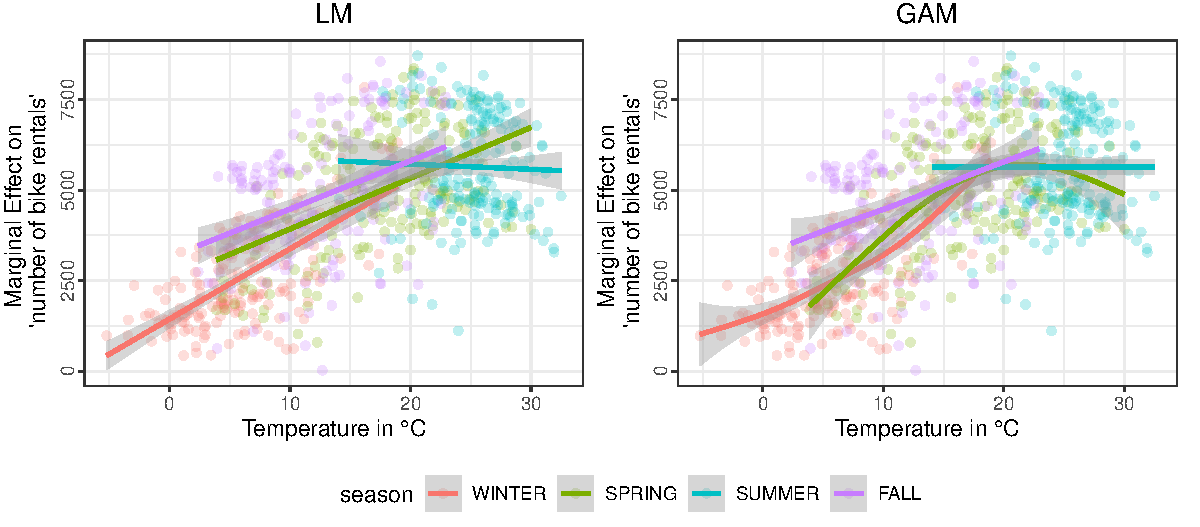
\includegraphics[width=0.75\textwidth, trim=0cm 0.1cm 0cm 0cm, clip]{\pathiml/figure/lm_main_interactions}}

\begin{itemize}
    \item Interactions: Feature effect is modified by other features and varies across observations \\ 
    $\Rightarrow$ Effect of temperature varies across seasons\\
    $\Rightarrow$ Multiple values / curves needed to describe effect
    \item ML models often model non-linear effects and complex interactions \\
    $\Rightarrow$ Need for local feature effect methods, e.g., analyze effect for individual observations\\
    $\Rightarrow$ Analyzing global effects by aggregating local effects
\end{itemize}




\end{frame}

%
% \begin{frame}{Feature Effects}
%
% %If the model contains interactions, the global effect is not enough as the
% %If the model contains interactions, there is a modifying effect for certain observations that changes the slope of the regression line (in case of LMs) or the shape of the partial effect curve (in case of GAMs).
% %(in case of LMs) or the shape of the partial effect curve (in case of GAMs).
% %If the model contains interactions, the slope of the regression line (in case of LMs) or the shape of the partial effect curve (in case of GAMs) will be different for certain observations.
% If the model contains interactions, the functional shape of the estimated feature effect will usually be different for certain observations.
% \lz
%
% \textbf{Example}: If we include the interaction \texttt{temp*season},
% %the marginal effect of \texttt{temp} will depend on \texttt{season}. That is,
% observations belonging to a certain category of \texttt{season} will have different marginal effects (slopes) for \texttt{temp}.
% %, which results in a different slope for the feature temp at each category of the feature season.
% %so that each category of season yields a different slope for temp.
%
% {\centering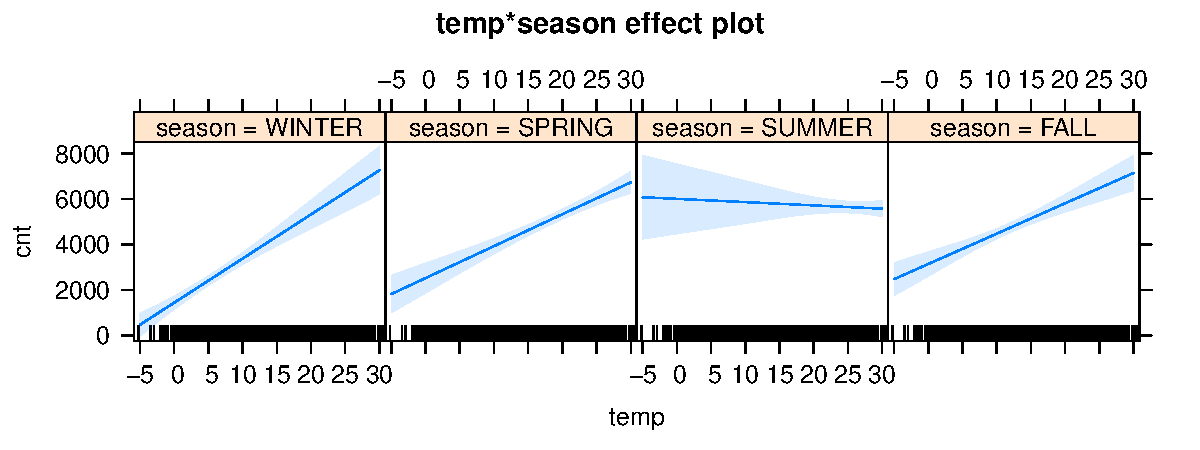
\includegraphics[width=0.9\textwidth, trim=0cm 0.1cm 0cm 0cm, clip]{figure_man/lm_interaction}}
%
% %\textbf{Note}: In case of interactions between two continuous features, we would obtain multiple regression lines with different slopes.
% %The marginal effect can then be visualized in a 2d effect plot or
%
% \end{frame}



\begin{frame}{Feature Effects}

\textbf{Feature effects} visualize or quantify marginal contribution of a feature of interest w.r.t. predictions %marginal contribution of a feature to the model \textbf{prediction}. % $\hat{y} = \fh(\xi[])$. effect (e.g., the average relationship) between a
\begin{itemize}
%\tightlist
\item Similar to regression coefficients (LMs) or Splines (GAMs)
\item Different aggregation levels for feature effects exist (simplification but information loss)
\item Methods: \visible<1-3>{ICE curves (local curves)}\visible<2-3>{, PD and ALE plots (global curves)}\visible<3>{, AME (global value)}
\end{itemize}

%\centerline{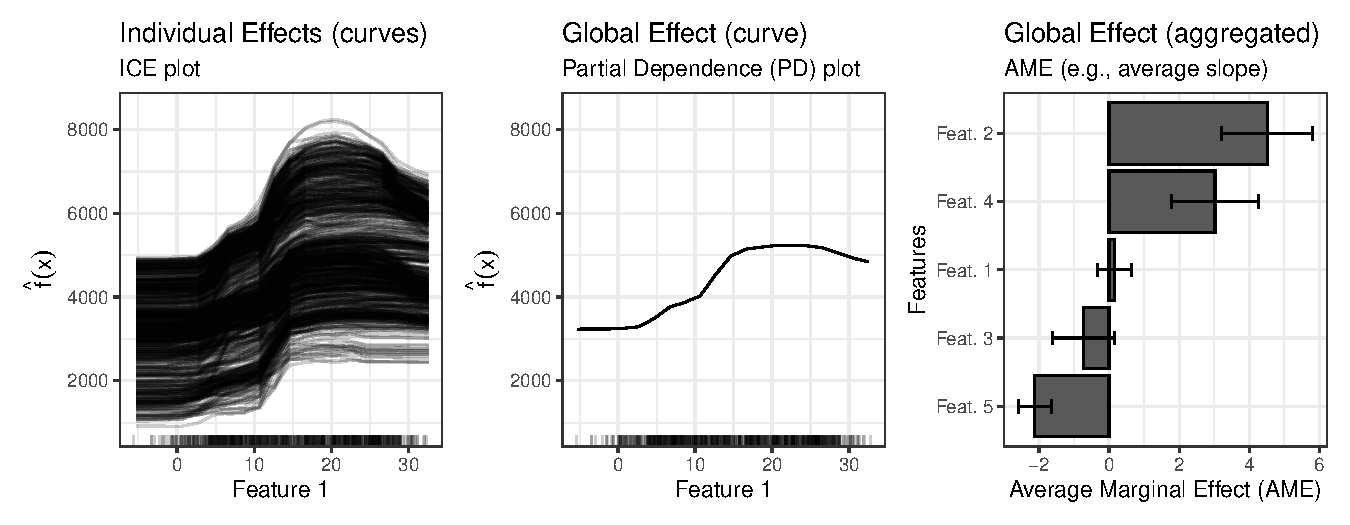
\includegraphics[width=\textwidth]{figure/feature-effect.pdf}}
\centerline{
\visible<1-3>{\adjincludegraphics[width=0.32\textwidth, trim={0 0 {.6667\width} 0}, clip]{\pathiml/figure/feature-effect.pdf}}
\visible<2-3>{\adjincludegraphics[width=0.32\textwidth, trim={{.33\width} 0 {.33\width} 0}, clip]{\pathiml/figure/feature-effect.pdf}}
\visible<3>{\adjincludegraphics[width=0.32\textwidth, trim={{.6667\width} 0 0 0}, clip]{\pathiml/figure/feature-effect.pdf}}
}

%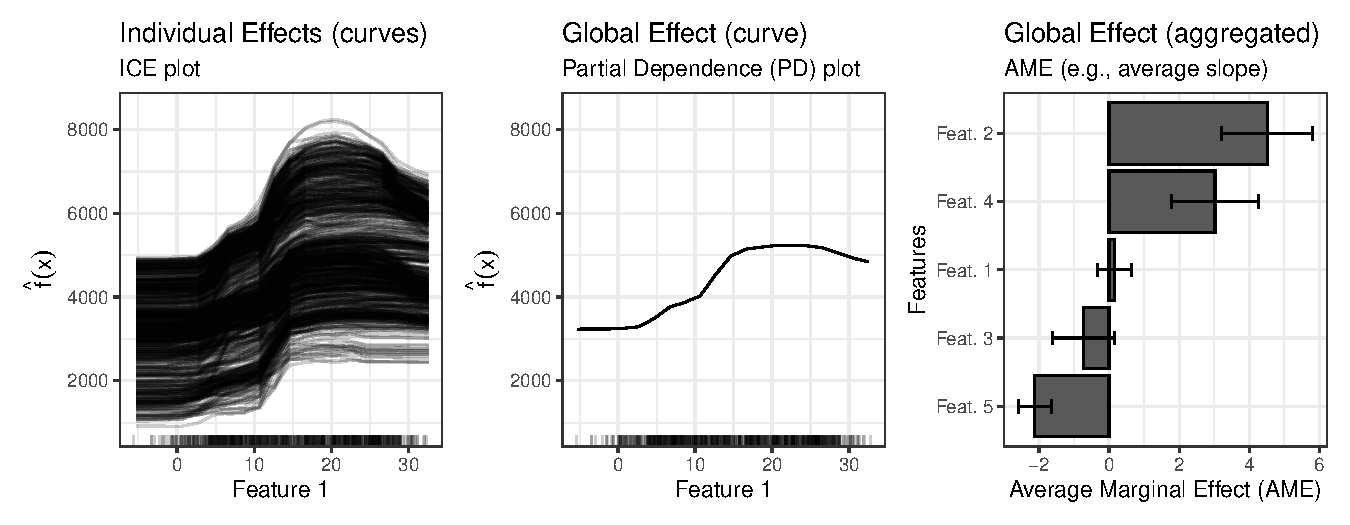
\includegraphics[width=0.33\textwidth, trim=7.4cm 0.1cm 7.4cm 0cm, clip]{figure/feature-effect.pdf}
%\invisible<1>{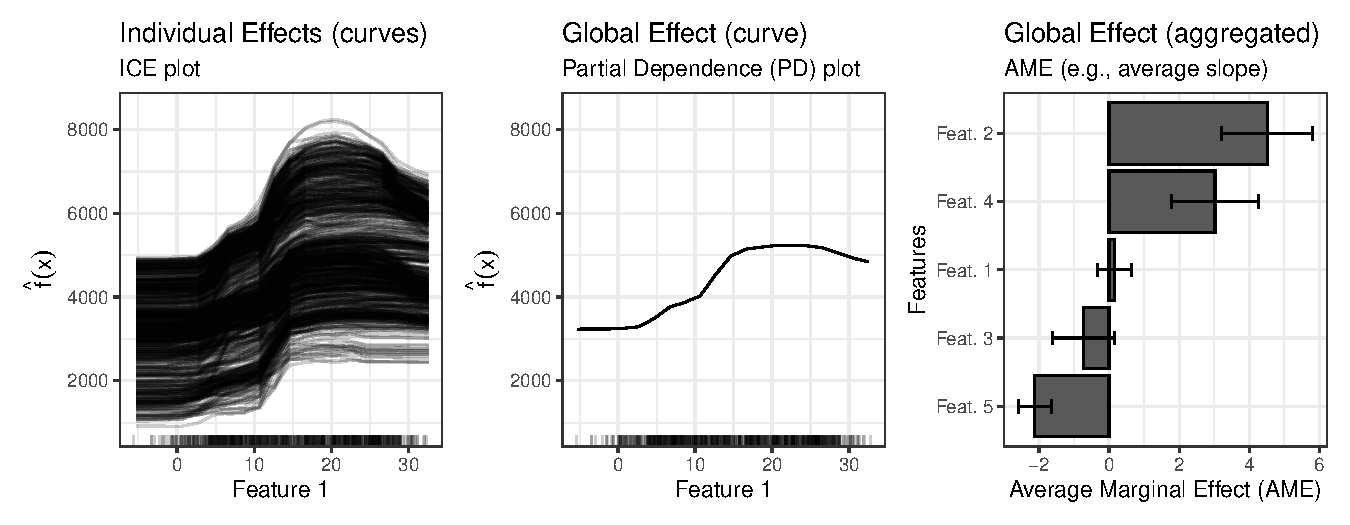
\includegraphics[width=0.33\textwidth, trim=14cm 0.1cm 0.4cm 0cm, clip]{figure/feature-effect.pdf}}

\centerline{\small \hspace{30px} \visible<1-3>{Individual (curves) \hspace{6px}}
\visible<2-3>{$\xrightarrow[\text{curves}]{\text{aggregate}}$ \hspace{6px} Global (single curve)}\visible<3>{\hspace{6px}
$\xrightarrow[\text{slopes}]{\text{aggregate}}$ \hspace{6px} Global (single value)}}


\end{frame}

%%%%%%%%%%%%%%%%%%%%%%%%%%%%%%%%%%%%%%%%%%%%%%%%%%%%%%%%%%%%%
\renewcommand{\titlefigure}{\pathiml/figure/feature-effect}
\renewcommand{\learninggoals}{
%\item Intro to feature effects
\item ICE curves as local effect method
\item How to sample grid points for ICE curves
%\item Understand how to interpret ICE curves and PD plots
}

\lecturechapter{Individual Conditional Expectation (ICE) Plot}
%\lecture{Interpretable Machine Learning}

\mysectionslide

\begin{frame}{Motivation}
%ICE curves show how different feature values of an observation affect its model prediction \newline $\Rightarrow$ \textbf{local interpretation method}
%From a local perspective, one might be interested in how changing feature values of an observation affect model prediction

\textbf{Question:} How does changing values of a single feature of an observation affect model prediction?

\smallskip

\textbf{Idea:} Change values of observation and feature of interest, and visualize how prediction changes

\smallskip

\textbf{Example:} Prediction surface of a model (left), select observation and visualize changes in prediction for different values of $x_2$ while keeping $x_1$ fixed $\Rightarrow$ \textbf{local interpretation}

\centering
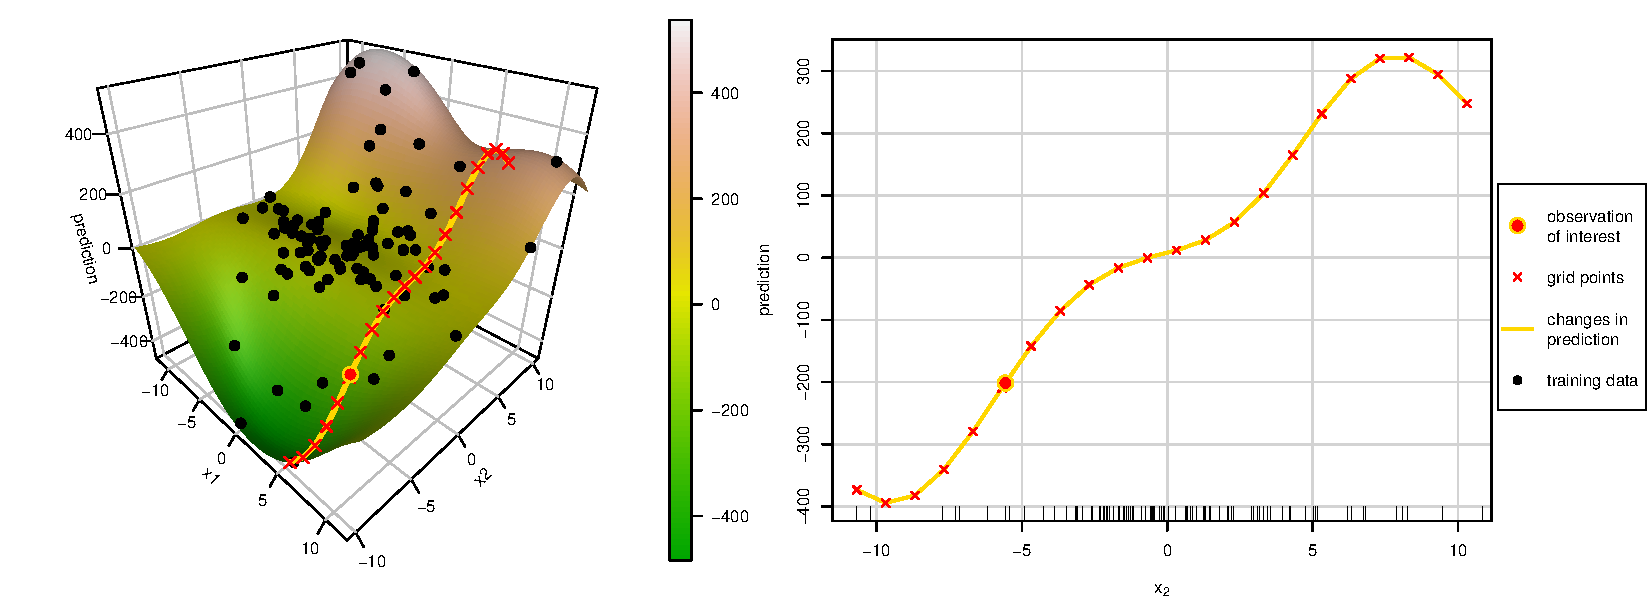
\includegraphics[width=0.85\textwidth]{\pathiml/figure/ice_motivation}

%$\Rightarrow$ Repeat for all observations and average the curves for global feature effect ($\leadsto$ PD plots)
\end{frame}




\begin{frame}[c]{Individual Conditional Expectation (ICE) \citebutton{Goldstein et. al (2013)}{https://doi.org/10.1080/10618600.2014.907095}}

%Consider an index set $S \subseteq \{1, \dots, p\}$ and its complement $C = S^\complement$.
%\lz
\begin{columns}[T]
\begin{column}{0.16\textwidth} % 0.2 4.26cm
\includegraphics[page=1, trim=0cm 0.35cm 4.53cm 0.35cm, clip, width=0.9\textwidth]{\pathiml/figure_man/ice_plot_demo}
\end{column}
\begin{column}{0.84\textwidth}

%%%

%Assume each observation $\xi$ can be partitioned into $\xi_S$ and $\xi_C$ containing only feature values from the index set $S \subseteq \{1, \dots, p\}$ and its complement $C = S^\complement$, respectively.
%Assume each observation $\xi$ can be partitioned into $\xi_S$ and $\xi_C$ containing only feature values addressed by the feature's index set $S \subseteq \{1, \dots, p\}$ and its complement $C = S^\complement$, respectively.
%Assume each observation $\xi$ can be partitioned into $\xi_S$ and $\xi_C$ containing values from features addressed by the index set $S \subseteq \{1, \dots, p\}$ and its complement $C = S^\complement$, respectively.
Partition each observation $\xv$ into $\xv_S$ (features of interest) and $\xv_{-S}$ (remaining feat.)
\begin{itemize}
    \item[$\leadsto$] In practice, $\xv_S$ consists of one or two features (i.e., $|S| \leq 2$ and ${-S} = S^\complement$).
    %, containing only feature values indexed by $S \subseteq \{1, \dots, p\}$ and its complement $C = S^\complement$.
\end{itemize}

\bigskip

Formal definition of ICE curves: 
\begin{itemize}
    \item Choose grid points $\xv_S^* = \xv_S^{*^{(1)}}, \dots, \xv_S^{*^{(g)}}$ to vary $\xv_S$
    \item Plot point pairs $ \Bigl\{\left(\xv_S^{*^{(k)}}, \fh_S^{(i)}(\xv_S^{*^{(k)}}) \right) \Bigr\}_{k=1}^g $ where $\fh_{S}^{(i)}(\xv_S^*) = \fh(\xv_S^*, \xi_{-S})$
    \item For each $k$ connect point pairs to obtain \textbf{ICE curve}
\end{itemize}

\bigskip

\begin{itemize}
    \item[$\leadsto$] ICE curves visualize how prediction of $i$-th observation changes after varying its feature values indexed by $S$ using grid points $\xv_S^*$ while keeping all values in $-S$ fixed:
%by replacing the feature values $\xv_S^{(i)}$ with other values $\xv_S$ while keeping all other features in $\xi_C$ fixed:
%by varying the feature values in $\xv_S$ while keeping all other features in $\xi_C$ fixed.

% \begin{itemize}
%     \item[$\leadsto$] Plot \quad $\fh_{S}^{(i)}(\xv_S^*) \; \text{ vs. } \; \xv_S^*$ \\
%     where $\fh_{S}^{(i)}(\xv_S^*) = \fh(\xv_S^*, \xi_{-S})$ is prediction of $i$-th observation in which original feature value $\xi_S$ was replaced by $\xv_S^*$.
% \end{itemize}
\end{itemize}


%Visualize for \textbf{I}ndividual observations and \textbf{C}onditional on all other features how \textbf{E}xpected prediction changes

\end{column}
\end{columns}

% \begin{columns}[T, totalwidth=\textwidth]
% \begin{column}{0.6\textwidth}


% \end{column}
% \begin{column}{0.4\textwidth}
% %\begin{center}
% \centerline{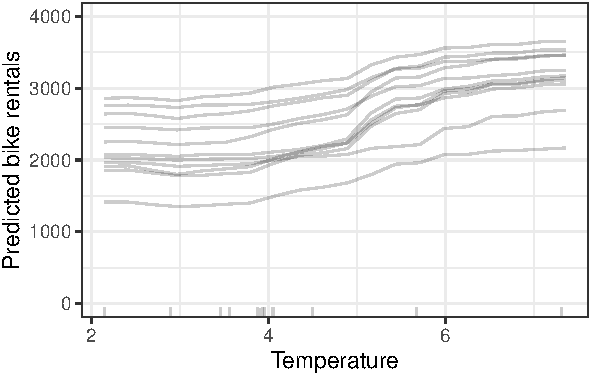
\includegraphics[width=\textwidth]{figure_man/ice_bike10obs}}
% %\end{center}
% %\vspace{-0.3cm}
% \scriptsize{\textbf{Figure:} ICE Curves of 10 observations of the bike sharing dataset. Each line displays the change in prediction for a single observation due to varying the feature temperature.\par}
%
% \end{column}
% \end{columns}
%\footnote[frame]{Goldstein, A., Kapelner, A., Bleich, J., and Pitkin, E. (2013). Peeking Inside the Black Box: Visualizing Statistical Learning with Plots of Individual Conditional Expectation, 1-22. https://doi.org/10.1080/10618600.2014.907095}
\end{frame}

% \begin{frame}{Individual Conditional Expectation (ICE)}
%
% Steps to create an ICE curve of an observation regarding a single feature $\xv_S$ according to the \textbf{SIPA} framework:
%
% \begin{enumerate}
% \item \textbf{Sampling:} Choose grid points along $\xv_S$.
% \item For each grid point:
% \begin{itemize}
% \item \textbf{Intervention:} Replace the original feature value $\xv_S$ with the current grid value.
% \item \textbf{Prediction:} Get the model prediction with replaced feature value $\xv_S$.
% \end{itemize}
% \item \textbf{Aggregation:} none.
% \item \textbf{Visualization:} Draw a curve per observation with the grid points on the x-axis and the prediction on the y-axis.
% \end{enumerate}
%
% \footnote[frame]{Scholbeck, C. A., Molnar, C., Heumann, C., Bischl, B., and Casalicchio, G. (2019). Sampling, Intervention, Prediction, Aggregation: A Generalized Framework for Model Agnostic Interpretations. ECML PKDD 2019. (pp. 205-216).}
% \end{frame}

% \begin{frame}{Individual Conditional Expectation (ICE)}
%
% \begin{columns}[T]
% \begin{column}{0.4\textwidth}
% \includegraphics[page=1, trim=0cm 0.35cm 0.85cm 0.35cm, width=0.9\textwidth]{figure_man/ice_plot_demo}
% \end{column}
% \begin{column}{0.55\textwidth}
%
% \end{column}
% \end{columns}
% %\vspace*{\topsep}
%
% aa
% \end{frame}

\begin{frame}{ICE Curves - Illustration}

\begin{columns}[T]
\begin{column}{0.4\textwidth}
\includegraphics[page=2, trim=0cm 0.35cm 0.85cm 0.35cm, width=0.9\textwidth]{\pathiml/figure_man/ice_plot_demo}
\end{column}
\begin{column}{0.55\textwidth}

\end{column}
\end{columns}
\vspace*{\topsep}

\textbf{1. Step - Grid points:}

%For the $i$-th observation, we
Sample grid values $\xv_S^{*^{(1)}}, \dots, \xv_S^{*^{(g)}}$ along feature of interest $\xv_S$
%
and replace vector $\xv^{(i)}$ in data with grid
%h observation with these sampled grid values.
%$\Rightarrow$ New artificial data points for $i$-th observation.
\newline $\Rightarrow$ Creates new artificial points for the $i$-th observation (here: $\xv_S^* = x_1^* \in \{1, 2, 3\}$ is a scalar)

\end{frame}

\begin{frame}{ICE Curves - Illustration}

\begin{columns}[T]
\begin{column}{0.4\textwidth}
\includegraphics<1>[page=3, trim=0cm 0.35cm 0.85cm 0.35cm, width=0.9\textwidth]{\pathiml/figure_man/ice_plot_demo}
\includegraphics<2>[page=4, trim=0cm 0.35cm 0.85cm 0.35cm, width=0.9\textwidth]{\pathiml/figure_man/ice_plot_demo}
\includegraphics<3>[page=5, trim=0cm 0.35cm 0.85cm 0.35cm, width=0.9\textwidth]{\pathiml/figure_man/ice_plot_demo}
\end{column}
\begin{column}{0.55\textwidth}
\includegraphics<1>[page=1, width=0.85\textwidth]{\pathiml/figure/ICE}
\includegraphics<2>[page=2, width=0.85\textwidth]{\pathiml/figure/ICE}
\includegraphics<3>[page=3, width=0.85\textwidth]{\pathiml/figure/ICE}
\end{column}
\end{columns}
\vspace*{\topsep}

\textbf{2. Step - Predict and visualize:}

For each artificially created data point of $i$-th observation, plot prediction $\fh_{S}^{(i)}(\xv_S^*)$ vs. grid values $\xv_S^*$:

$$\fh_{1}^{(i)}(x_1^*) = \fh(x_1^*, \xi_{2, 3}) \text{ vs. } x_1^* \in \{1, 2, 3\}$$

\end{frame}

% \begin{frame}{Individual Conditional Expectation (ICE)}

% \begin{columns}[T]
% \begin{column}{0.4\textwidth}
% \includegraphics[page=4, trim=0cm 0.35cm 0.85cm 0.35cm, width=0.9\textwidth]{figure_man/ice_plot_demo}
% \end{column}
% \begin{column}{0.55\textwidth}
% \includegraphics[page=2, width=0.85\textwidth]{figure/ICE}
% \end{column}
% \end{columns}
% \vspace*{\topsep}

% \textbf{Predict and visualize:}

% For each artificially created data point of $i$-th observation, plot prediction $\fh_{S}^{(i)}(\xv_S^*)$ vs. grid values $\xv_S^*$:

% $$\fh_{1}^{(i)}(x_1^*) = \fh(x_1^*, \xi_{2, 3}) \text{ vs. } x_1^* \in \{1, 2, 3\}$$
% \end{frame}

% \begin{frame}{Individual Conditional Expectation (ICE)}

% \begin{columns}[T]
% \begin{column}{0.4\textwidth}
% \includegraphics[page=5, trim=0cm 0.35cm 0.85cm 0.35cm, width=0.9\textwidth]{figure_man/ice_plot_demo}
% \end{column}
% \begin{column}{0.55\textwidth}
% \includegraphics[page=3, width=0.85\textwidth]{figure/ICE}
% \end{column}
% \end{columns}
% \vspace*{\topsep}

% \textbf{Predict and visualize:}

% For each artificially created data point of $i$-th observation, plot prediction $\fh_{S}^{(i)}(\xv_S^*)$ vs. grid values $\xv_S^*$:

% $$\fh_{1}^{(i)}(x_1^*) = \fh(x_1^*, \xi_{2, 3}) \text{ vs. } x_1^* \in \{1, 2, 3\}$$
% \end{frame}

% \begin{frame}{Individual Conditional Expectation (ICE)}

% % \begin{columns}[T]
% % \begin{column}{0.4\textwidth}
% % \includegraphics[page=5, trim=0cm 0.35cm 0.85cm 0.35cm, width=0.9\textwidth]{figure_man/ice_plot_demo}
% % \end{column}
% % \begin{column}{0.55\textwidth}
% % \includegraphics[page=3, width=0.85\textwidth]{figure/ICE}
% % \end{column}
% % \end{columns}
% % \vspace*{\topsep}

% \begin{itemize}
%     \item \textbf{Interpretation:} \textbf{ICE} curve visualizes for \textbf{I}ndividual observations and \textbf{C}onditional on all other features (by keeping all other features constant) how \textbf{E}xpected prediction changes
%     \item
%     \item For global view, repeat procedure for all observations
% \end{itemize}

% % \textbf{Definition:}

% % ICE curves involve plotting the pairs $ \{(\xv_S^{*^{(k)}}, \fh_{S}^{(i)}(\xv_S^*{^{(k)}})) \}_{k=1}^g $ for grid points $\xv_S^{*^{(1)}}, \dots, \xv_S^{*^{(g)}}$.
% \end{frame}

\begin{frame}{ICE Curves - Illustration}

\begin{columns}[T]
\begin{column}{0.4\textwidth}
\includegraphics<1>[page=6, trim=0cm 0.35cm 0.85cm 0.35cm, width=0.9\textwidth]{\pathiml/figure_man/ice_plot_demo}
\includegraphics<2>[page=7, trim=0cm 0.35cm 0.85cm 0.35cm, width=0.9\textwidth]{\pathiml/figure_man/ice_plot_demo}
\end{column}
\begin{column}{0.55\textwidth}
\includegraphics<1>[page=4, width=0.85\textwidth]{\pathiml/figure/ICE}
\includegraphics<2>[page=5, width=0.85\textwidth]{\pathiml/figure/ICE}
\end{column}
\end{columns}
\vspace*{\topsep}

\textbf{3. Step - Repeat for other observations:}

ICE curve for\only<1>{ $i=2$ }\only<2>{ $i=3$ }connects all predictions at grid values associated to $i$-th observation.
\end{frame}

% \begin{frame}{ICE Curves - Illustration}

% \begin{columns}[T]
% \begin{column}{0.4\textwidth}
% \includegraphics[page=7, trim=0cm 0.35cm 0.85cm 0.35cm, width=0.9\textwidth]{figure_man/ice_plot_demo}
% \end{column}
% \begin{column}{0.55\textwidth}
% %\begin{center}
% \includegraphics[page=5, width=0.85\textwidth]{figure/ICE}
% %\end{center}
% \end{column}
% \end{columns}
% \vspace*{\topsep}

% \textbf{3. Step - Repeat for other observations:}

% ICE curve for $i=3$ connects all predictions at grid values associated to $i$-th observation.
% %The ICE curve of observation $i=3$ connects all predictions at the corresponding grid values associated to the $i$-th observation.

% % \textbf{Definition:}

% % ICE curves involve plotting the pairs $ \{(\xv_S^{*^{(k)}}, \fh_{S}^{(i)}(\xv_S^*{^{(k)}})) \}_{k=1}^g $ for grid points $\xv_S^{*^{(1)}}, \dots, \xv_S^{*^{(g)}}$.
% \end{frame}


% \begin{frame}{Comments on Grid values}
% \begin{itemize}
% %\item ICE curves show how different feature values of an observation affect its prediction \newline $\Rightarrow$ \textbf{local interpretation method}
% \item Plotting ICE curves involves generating grid values $\xv_S^*$ that are visualized on the x-axis
% \item Common choices for grid values are
% \begin{itemize}
% \item equidistant grid values within feature range
% \item randomly sampled values or quantile values of observed feature values
% \end{itemize}
% \item Except equidistant grid, the other two options preserve (approximately) the marginal distribution of feature of interest
% $\Rightarrow$ Avoids unrealistic feature values for distributions with outliers %or dependencies

% \vspace{3pt}
% \centering
% 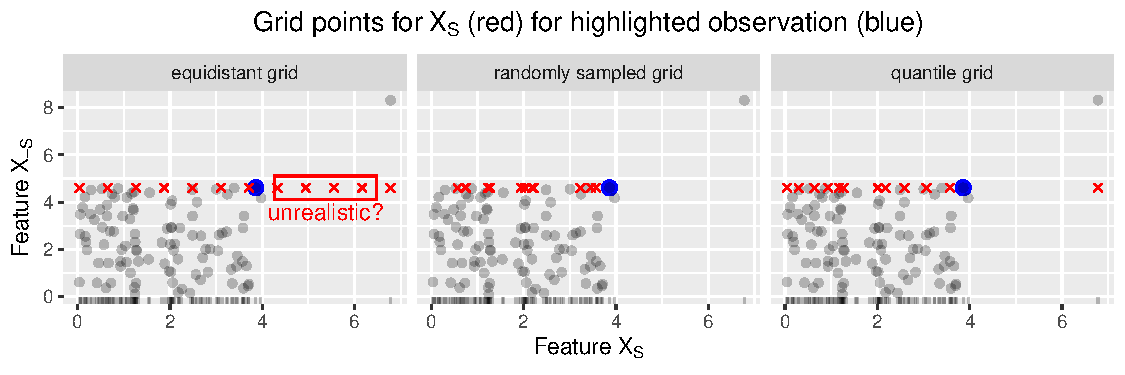
\includegraphics[width=0.75\textwidth, trim=0cm 0cm 0cm 0cm, clip]{\pathiml/figure/sampling2}

% %Preferable for skewed distributions (with outliers) to avoid using unrealistic feature values.
% % \begin{itemize}
% % \item equidistant grid values:
% % \item sub-sampled grid values:
% % \item quantile grid values:
% % \end{itemize}
% \end{itemize}
% \end{frame}


\begin{frame}{Comments on Grid values}
\begin{itemize}
%\item ICE curves show how different feature values of an observation affect its prediction \newline $\Rightarrow$ \textbf{local interpretation method}
\item Plotting ICE curves involves generating grid values $\xv_S^*$ that are visualized on the x-axis
\item Common choices for grid values are
\begin{itemize}
\item equidistant grid values within feature range
\item randomly sampled values or quantile values of observed feature values
\end{itemize}
\item Except equidistant grid, the other two options preserve (approximately) the marginal distribution of feature of interest
$\Rightarrow$ Avoids unrealistic feature values for distributions with outliers %or dependencies

\vspace{3pt}
\centering
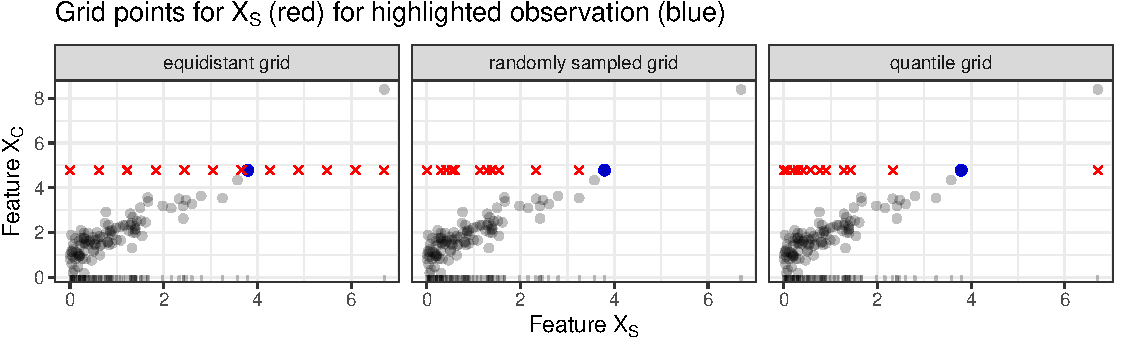
\includegraphics[width=0.75\textwidth, trim=0cm 0cm 0cm 0cm, clip]{\pathiml/figure/sampling}

%Preferable for skewed distributions (with outliers) to avoid using unrealistic feature values.
% \begin{itemize}
% \item equidistant grid values:
% \item sub-sampled grid values:
% \item quantile grid values:
% \end{itemize}
\end{itemize}
\end{frame}


%%%%%%%%%%%%%%%%%%%%%%%%%%%%%%%%%%%%%%%%%%%%%%%%%%%%%%%%%%%%
%%%%%%%%%%%%%%%%%%%%%%%%%%%%%%%%%%%%%%%%%%%%%%%%%%%%%%%%%%
\renewcommand{\titlefigure}{\pathiml/figure/pdp_bike}
\renewcommand{\learninggoals}{
\item PD plots and relation to ICE plots
\item Interpretation of PDP
\item Extrapolation and Interactions in PDPs
\item Centered ICE and PDP
}

\lecturechapter{Partial Dependence (PD) plot}
%\lecture{Interpretable Machine Learning}
\mysectionslide


\begin{frame}{Partial Dependence (PD) \citebutton{Friedman (2001)}{https://www.jstor.org/stable/2699986}}

\textbf{Definition:} PD function is expectation of $\fh(\xv_S, \xv_{-S})$ w.r.t. marginal distribution of features $\xv_{-S}$:
$$f_{S, PD}(\xv_S) = \E_{\xv_{-S}} \left( \fh(\xv_S, \xv_{-S}) \right) = \int_{-\infty}^{\infty} \fh(\xv_S, \xv_{-S}) \, d\P(\xv_{-S})$$

\textbf{Estimation:} For a grid value $\xv_S^*$, average ICE curves point-wise at $\xv_S^*$ over all observed $\xv_{-S}^{(i)}$:
$$\fh_{S, PD}(\xv_S^*) = \frac{1}{n} \sum_{i=1}^n \fh(\xv_S^*, \xv_{-S}^{(i)})$$

%Within the SIPA framework, the partial dependence builds the \textbf{Aggregation} step.

%\footnote[frame]{Friedman, Jerome H. (2001). Greedy Function Approximation: A Gradient Boosting Machine. Annals of Statistics: 1189-1232.}
%\footnote[frame]{Scholbeck, C. A., Molnar, C., Heumann, C., Bischl, B., and Casalicchio, G. (2019). Sampling, Intervention, Prediction, Aggregation: A Generalized Framework for Model Agnostic Interpretations. ECML PKDD 2019. (pp. 205-216).}
\end{frame}


% \frame{
% \frametitle{Example: Partial Dependence for Linear Model}

% Assume a linear regression model with two features:

% $$\fh(\xv) = \fh(\xv_1, \xv_2) = \hat\theta_1 \xv_1 + \hat\theta_2 \xv_2 + \hat\theta_0$$

% PD function for feature of interest $S = \{1\}$ (with $-S = \{2\}$) is:

% $$
% \begin{aligned}
% f_{1, PD}(\xv_1) = \E_{\xv_2} \left( \fh(\xv_1, \xv_2) \right) &= \int_{-\infty}^{\infty} \left( \hat\theta_1 \xv_1 + \hat\theta_2 \xv_2 + \hat\theta_0 \right) \, d\P(\xv_2) \\
% &= \hat\theta_1 \xv_1 + \hat\theta_2 \cdot \int_{-\infty}^{\infty} \xv_2 \, d\P(\xv_2) + \hat\theta_0 \\
% &= \hat\theta_1 \xv_1 + \underbrace{\hat\theta_2 \cdot \E_{\xv_2} (\xv_2) + \hat\theta_0}_{:= const}
% \end{aligned}
% $$

% $\Rightarrow$ PD plot visualizes the function $f_{1, PD}(\xv_1) = \hat\theta_1 \xv_1 + const$ ($\hat =$ feature effect of $\xv_1$).

% }

\frame{
\frametitle{Partial Dependence}
%\begin{onlyenv}
\begin{columns}[T]
\begin{column}{0.5\textwidth}
\centering
\only<1>{
\includegraphics[page=8, width=0.8\textwidth]{\pathiml/figure_man/ice_pd_plot_demo}
\end{column}
\begin{column}{0.5\textwidth}

\begin{center}
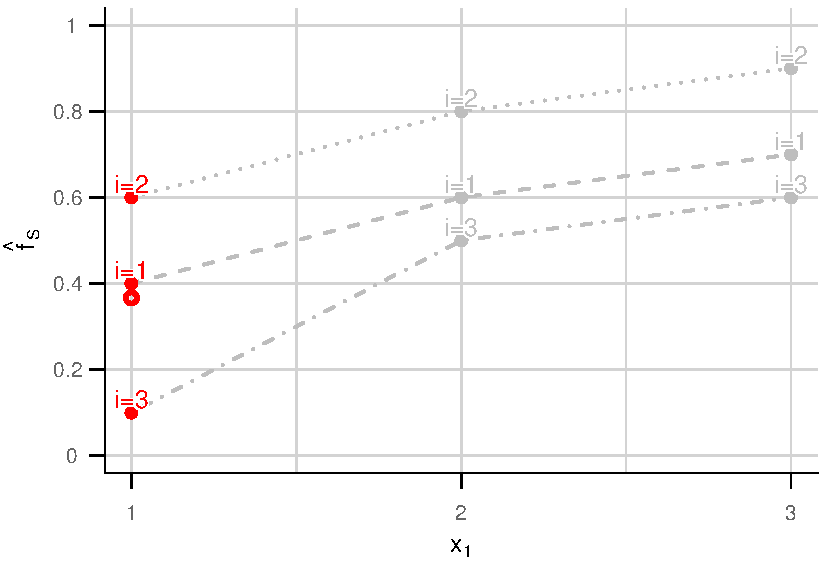
\includegraphics[page=1, width=\textwidth]{\pathiml/figure/PD}
\end{center}
}

\only<2>{
\includegraphics[page=9, width=0.8\textwidth]{\pathiml/figure_man/ice_pd_plot_demo}
\end{column}
\begin{column}{0.5\textwidth}

\begin{center}
\includegraphics[page=2, width=\textwidth]{\pathiml/figure/PD}
\end{center}
}

\only<3>{
\includegraphics[page=10, width=0.8\textwidth]{\pathiml/figure_man/ice_pd_plot_demo}
\end{column}
\begin{column}{0.5\textwidth}

\begin{center}
\includegraphics[page=3, width=\textwidth]{\pathiml/figure/PD}
\end{center}
}
\end{column}
\end{columns}
%\end{onlyenv}

Estimate PD function by \textbf{point-wise} average of ICE curves at grid value \fcolorbox{red}{white}{$\xv_S^* = x_1^* = \only<1>{1}\only<2>{2}\only<3>{3}$}:
$$\textstyle\fh_{1, PD}(x_1^*) = \frac{1}{n} \sum_{i=1}^n \fh(x_1^*, \xv_{2, 3}^{(i)})$$
}


\frame{
\frametitle{Interpretation: PD and ICE}

If feature varies:\\
\begin{itemize}
\item
  \textbf{ICE:} How does \textbf{prediction of
  individual observation} change? \(\Rightarrow\) \textbf{local} interpretation
\item
  \textbf{PD:} How does \textbf{average effect / expected prediction} change? \(\Rightarrow\) \textbf{global} interpretation
\end{itemize}

\begin{columns}[c]
\begin{column}{0.6\textwidth}
\begin{center}
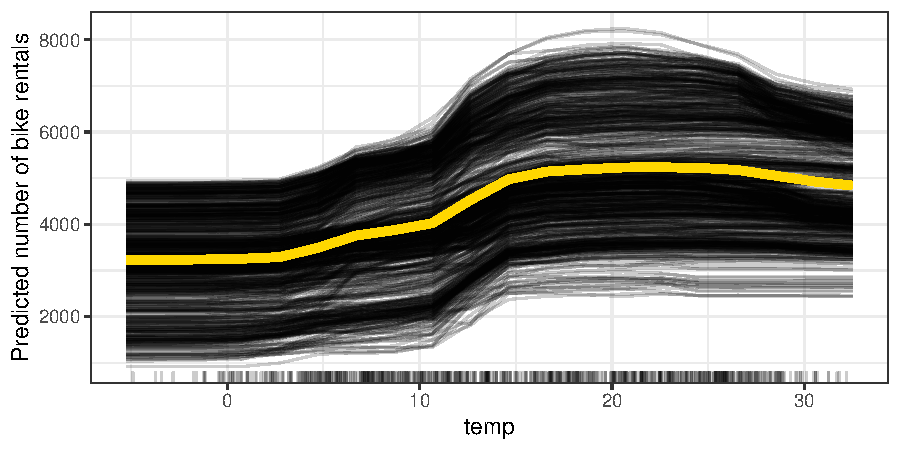
\includegraphics[width=\textwidth]{\pathiml/figure/pdp_bike}
\end{center}
\end{column}
%\pause
\begin{column}{0.4\textwidth}
Insights from bike sharing data:
\begin{itemize}
%  \item Averaging ICE curves yields PD plot (yellow curve)
  \item Parallel ICE curves = homogeneous effect
  \item Warmer $\Rightarrow$ more rented bikes
  \item Too hot $\Rightarrow$ slightly less bikes 
\end{itemize}
\end{column}
\end{columns}
}


\frame{
\frametitle{Interpretation: Categorical Features}

\begin{center}
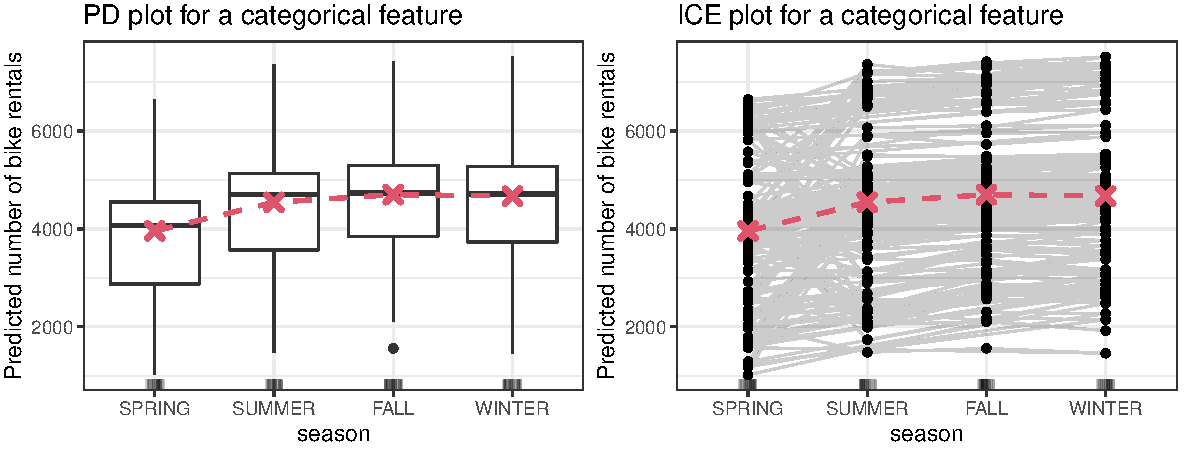
\includegraphics[width=0.9\textwidth]{\pathiml/figure/pdp_ice_cat}
\end{center}

\begin{itemize}
\item PDP with boxplots and ICE with parallel coordinates plots
%lot visualizes expected prediction if all observations would belong to a certain category (and shows distribution of predictions in a box plot)
\item NB: Categories can be unordered, if so, rather compare pairwise
\end{itemize}
%ICE plot connects predictions of individual observations (might identify heterogenous effects between categories if many lines are crossing)\\
%to identify heterogenous effects between categories (here: lines between SPRING and SUMMER are heterogenous).\\

}


% \begin{frame}{Comments on Extrapolation}

% % \begin{center}
% % 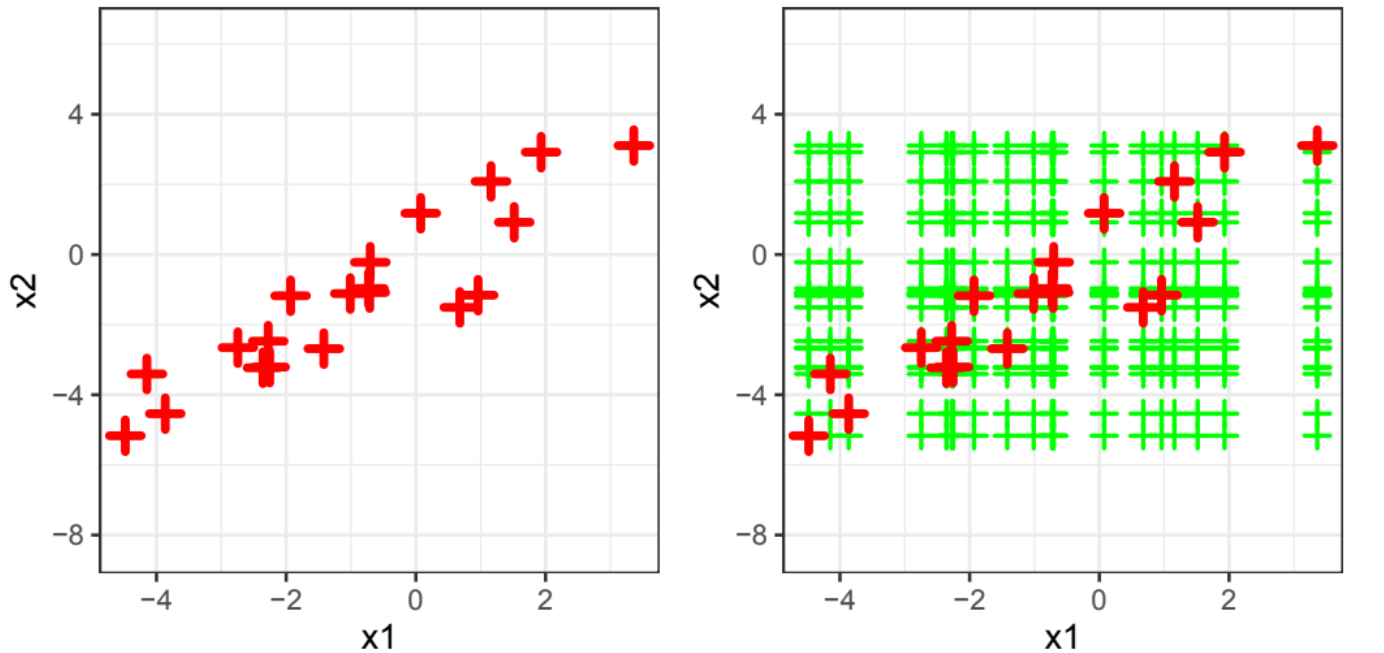
\includegraphics[width=0.8\textwidth]{figure_man/extrapolation01.png}
% % \end{center}

% Extrapolation can cause issues in regions with few observations or if features are correlated
 
% \begin{columns}[T]
% \begin{column}{0.5\textwidth}
% \centering
% \includegraphics[width=0.8\textwidth]{\pathiml/figure/ale_scatter_grid}
% \end{column}
% \begin{column}{0.5\textwidth}
% \centering
% \includegraphics[width=0.8\textwidth]{\pathiml/figure/ale_pdplot}
% \end{column}
% \end{columns}

% \begin{itemize}
% \item \textbf{Example:} Features $x_1$ and $x_2$ are strongly correlated
% \item \textbf{Black points:} Observed points of the original data
% \item \textbf{\textcolor{red}{Red:}} Grid points used to calculate the ICE and PD curves (several unrealistic values)\\ %combination of feature values
% $\Rightarrow$ %Unrealistic combination of feature values are used, e.g., the
% PD plot at $x_1=0$ averages predictions over the whole marginal distribution of feature $x_2$\\
% $\Rightarrow$ May be problematic if model behaves strange outside training distribution
% %can bias ICE and PD curves Be careful with interpretations 
% %\item For correlated features and in regions with few observations with care
% %Extrapolation: interpret curves for highly correlated features and in feature regions with few observations with care
% \end{itemize}

% %
% % \framebreak
% %
% %
% % \begin{center}
% % \includegraphics[width=0.8\textwidth]{figure_man/extrapolation02.png}
% % \end{center}
% %
% % \begin{itemize}
% % \item The features $x_1$ and $x_2$ are strongly correlated.
% % \item \textcolor{red}{Red:} Observed points of the original data.
% % \item \textcolor{green}{Green:} Grid points used to calculate the ICE and PD curves.
% % \item Example: PD plot at $x_1=1.9$ averages predictions over the whole marginal distribution of feature $x_2$.
% % \end{itemize}
% \end{frame}




% \begin{frame}{Interactions}
%
% For PD plots, the averaging of ICE curves might \textbf{obfuscate} heterogeneous effects and interactions. \newline \(\Rightarrow\) Ideally plot ICE curves and PD plots together.
%
% \begin{center}\includegraphics[width=0.65\textwidth]{figure_man/pdp_xor.pdf} \end{center}
% %
% % \framebreak
% %
% % \begin{itemize}
% % \item
% %   For PD plots, the averaging of ICE curves might \textbf{obfuscate}
% %   heterogeneous effects and interactions. \newline \(\Rightarrow\)
% %   Ideally plot ICE curves and PD plots together.
% % \item
% %   \textbf{Extrapolation:} Interprete curves for highly correlated
% %   features and in feature regions with few observations with care.
% % \item
% %   Accumulated Local Effects (ALE) plots are a novel alternative to the PD plots developed by Apley (2020) that do not suffer from
% %   extrapolation in case of correlated features.
% % \end{itemize}
% %
% % \vspace{80pt}
% % \tiny{
% % Apley, D. W., \& Zhu, J. (2020). Visualizing the effects of predictor variables in black box supervised learning models. Journal of the Royal Statistical Society: Series B, 82(4), 1059-1086. \par}
% \end{frame}

\begin{frame}{Comments on Interactions}
\begin{itemize}
%\lz
%\item Accumulated Local Effects (ALE) plots are a novel alternative to PD plots developed by Apley (2016) that do not suffer from extrapolation in case of correlated features.

\item PD plots: averaging of ICE curves might \textbf{obfuscate} heterogeneous effects and interactions \\ 
\(\Rightarrow\) Ideally plot ICE curves and PD plots together to uncover this fact\\
\(\Rightarrow\) Different shapes of ICE curves suggest interaction (but does not tell with which  feature)

\begin{center}\includegraphics[width=0.5\textwidth]{\pathiml/figure/pdp_xor.pdf} \end{center}
\end{itemize}

%\footnote[frame]{Apley, Daniel W., and Jingyu Zhu (2020). Visualizing the Effects of Predictor Variables in Black Box Supervised Learning Models. Journal of the Royal Statistical Society: Series B (Statistical Methodology) 82.4: 1059-1086.}
\end{frame}

% \begin{frame}{Comments on Interactions - 2D Partial Dependence}

% \begin{center}
% \includegraphics[width=0.9\textwidth]{\pathiml/figure/pdp2d_bike}
% \end{center}

% \begin{itemize}
%  \item Humidity and temperature interact with each other at high values (see shape difference)\\
%  $\leadsto$ Shape of ICE curves at different horizontal and vertical slices varies (for high values)
%  \item Low to medium humidity and high temperature $\Rightarrow$ many rented bikes
%  %Many rented bikesThe number of bike rentals is especially high when humidity is below 75 percent and temperature is between 15 $^{\circ}$C and 27 $^{\circ}$C
% \end{itemize}


% % \framebreak
% %
% % add datapoints to previous figure and mention convex hull (see pdp package)

% \end{frame}


\begin{frame}{Centered ICE Plot (c-ICE)}

\textbf{Issue:} Difficult to identify heterogenous ICE curves if curves have different intercepts (are stacked)
%When ICE curves start at different intercepts (are stacked), it is difficult to identify heterogenous predictions.

\textbf{Solution:} Center ICE curves at fixed reference value $x' \sim \P(\xv_S)$, often $x' = \min(\xv_S)$\\
$\Rightarrow$ Easier to identify heterogenous shapes with c-ICE curves
\vspace{-0.2cm}
\begin{columns}[c]
\begin{column}{0.4\textwidth}
%\centering
$$\begin{aligned}
\fh_{S, cICE}^{(i)}(\xv_S)
&= \fh(\xv_S, \xi_{-S}) - \fh(x', \xi_{-S}) \\
&= \fh_{S}^{(i)}(\xv_S) - \fh_{S}^{(i)}(x')
\end{aligned}$$

$\Rightarrow$ Visualize $\fh_{S, cICE}^{(i)}(\xv_S^*)$ vs. grid point $\xv_S^*$

\lz
\pause
\textbf{Interpretation} (yellow curve in c-ICE): \\
On average, the number of bike rentals at $\sim 97$ \% humidity decreased by 1000 bikes compared to a humidity of 0 \%
\end{column}
\begin{column}{0.59\textwidth}
\begin{center}
%\vspace{-0.3cm}
\includegraphics[width=\textwidth]{\pathiml/figure/cICE}
\end{center}
\end{column}
\end{columns}

%\vspace{-0.4cm}

\end{frame}


\begin{frame}{Centered ICE Plot (c-ICE)}

For categorical features, c-ICE plots can be interpreted as in LMs due to reference value

\begin{columns}[c]
\begin{column}{0.44\textwidth}

\begin{center}
\includegraphics[width=\textwidth]{\pathiml/figure/cICEcat}
\end{center}

\end{column}
\begin{column}{0.55\textwidth}

\textbf{Interpretation}: \\
\begin{itemize}
%\item Centered ICE plots are useful for categorical features and can be interpreted as in LMs
\item The reference category is $x' =$ SPRING
\item Golden crosses: Average number of bike rentals if we jump from SPRING to any other season\\
$\Rightarrow$ Number of bike rentals drops by $\sim 560$ in \code{WINTER} and is slightly higher in \code{SUMMER} and \code{FALL} compared to \code{SPRING}
\end{itemize}

\end{column}
\end{columns}

\end{frame}


%%%%%%%%%%%%%%%%%%%%%%%%%%%%%%%%%%%%%%%%%%%%%%%%%%%%%%%%%


\renewcommand{\titlefigure}{\pathiml/figure/ale_plot.pdf}
\renewcommand{\learninggoals}{
\item PD plots and its extrapolation issue
\item M plots and its omitted-variable bias
\item Understand ALE plots
}

\lecturechapter{Accumulated Local Effect (ALE) plot}
%\lecture{Interpretable Machine Learning}
\mysectionslide
%
% \frame{
% \frametitle{Motivation}
%
% \begin{columns}[T]
% \begin{column}{0.5\textwidth}
% \centering
% \includegraphics[width=\textwidth]{figure_man/ale_scatter}
% \end{column}
% \begin{column}{0.5\textwidth}
% \centering
% \includegraphics[width=\textwidth]{figure_man/ale_pdplot}
% \end{column}
% \end{columns}
%
% \only<1>{
% \textbf{Recall:} In case of strongly correlated features $x_1$ and $x_2$, partial dependence (PD) plots \textbf{average predictions} of artificial data instances that are unlikely in reality (green).
% This can lead to biased estimates.
%
% \textbf{Question:} Can we avoid the extrapolation issue by averaging only over points in an appropriate neighborhood? % of a specific point $x_1$? %, i.e., using the conditional distribution at
% }
%
% \only<2>{
%
% \textbf{Answer:} Yes, we could. Marginal plots (M plots) do this by averaging (i.e., marginalizing) over the conditional distribution $\P(\xv_2|x_1)$.
%
% \textbf{But:} M plots introduce the omitted-variable bias (OVB) issue, i.e., an
% M plot always includes the marginal effect of other dependent features.\\
% $\Rightarrow$ M plots are useless to assess the main effect of a feature.
%
% }
% }



\begin{frame}{Motivation - Correlated Features}

\begin{columns}[T]
\begin{column}{0.5\textwidth}
\centering
\includegraphics[width=0.9\textwidth]{\pathiml/figure/ale_scatter_grid}
\end{column}
\begin{column}{0.5\textwidth}
\centering
\includegraphics[width=0.9\textwidth]{\pathiml/figure/ale_pdplot}
\end{column}
\end{columns}

%\begin{center}
%\includegraphics[width=0.8\textwidth]{figure_man/pd_grid}
%\tiny{Source: Figure taken from Apley et al. (2020)}
%\end{center}

%In case of strongly correlated features $x_1$ and $x_2$, PD plots \textbf{average predictions} of artificial data points that are unlikely in reality (red).

\begin{itemize}
    \item PD plots \textbf{average over predictions} of artificial points that are out of distribution / unlikely (red)\\
    $\Rightarrow$ Can lead to misleading / biased interpretations, especially if model also contains interactions
    \item Not wanted if interest is to interpret effects within data distribution
\end{itemize}
%If features are correlated, PD plots \textbf{average predictions} of artificial points that are unlikely (red).
%\textbf{But:} This might be undesired if interest is to interpret effects within data distribution.
%This can be an undesired property if the model contains interactions and one is interested in interpreting effects w.r.t. the data distribution.

%\lz

%\textbf{Question:} Can we avoid the extrapolation issue by averaging only over points in an appropriate neighborhood? % of a specific point $x_1$? %, i.e., using the conditional distribution at

\end{frame}


\begin{frame}{Motivation - Correlated Features}

%TODO: Example what can go wrong with PDPs and NNs

Example: Fit a NN to $5000$ simulated data points with $x \sim Unif(0,1)$, $\epsilon \sim N(0, 0.2)$ and

\centerline{$y = x_1 + x_2^2 + \epsilon$, where
$x_1 = x + \epsilon_1$, 
$x_2 = x + \epsilon_2$ and $\epsilon_1, \epsilon_2 \sim N(0, 0.05)$.}

\begin{columns}[T]
\begin{column}{0.65\textwidth}
\centering
\only<1>{\includegraphics[width=\textwidth]{\pathiml/figure/ale_vs_pdp_surf}}
\only<2>{\includegraphics[width=\textwidth]{\pathiml/figure/ale_vs_pdp_nn}}
\end{column}
\begin{column}{0.35\textwidth}
%What went wrong here?

\begin{itemize}
\item Test error (MSE) of NN is comparable to other models
\item NN contains interactions (see complex pred. surface)
%\item ALE shows a linear effect for $x_1$ and quadratic effect for $x_2$\\
%$\Rightarrow$ In line with ground truth %Match true effects of DGP
%\item PDP shows expected model behaviour but does not recover effects of DGP \\
%$\Rightarrow$ Due to averaging of artificial points outside data distribution
\item<2> ALE in line with ground truth
\item<2> PDP does not reflect ground truth effects of DGP well \\
$\Rightarrow$ Due to interactions and averaging of points outside data distribution
\end{itemize}

\end{column}
\end{columns}

\end{frame}

\begin{frame}{M Plot vs. PD plot}

% \begin{center}
% \includegraphics[width=0.7\textwidth]{figure_man/PD_M.jpg}\\
% \tiny{Source: Figure taken from Apley et al. (2020)}
% \end{center}

\begin{columns}[T]
\visible<1-2>{\begin{column}{0.5\textwidth}
\vspace*{-1em}
\centering
\textbf{a) PD plot}
\includegraphics[width=0.9\textwidth]{\pathiml/figure/ale_pdplot}
\end{column}
}
\visible<2>{\begin{column}{0.5\textwidth}
\vspace*{-1em}
\textbf{b) M plot}
\centering
\includegraphics[width=0.9\textwidth]{\pathiml/figure/ale_mplot}
\end{column}
}
\end{columns}

\begin{enumerate}[<+->]
%\item[a)] PD plot $\fh_{1, PD}(x_1) = \hat{\E}_{\xv_2} \left( \fh(x_1, \xv_2) \right) = \frac{1}{n} \sum_{i=1}^n \fh(x_1, \xv_2^{(i)})$
%\item[b)] M plot $\fh_{1, M}(x_1) = \hat{\E}_{\xv_2|\xv_1} \left( \fh(x_1, \xv_2) \middle| \xv_1\right) = \frac{1}{|N(x_1)|} \sum\limits_{i \in N(x_1)} \fh(x_1, \xv_2^{(i)})$, where $N(x_1) = \{i: x_1^{(i)} \in [x_1 - \epsilon, x_1 + \epsilon]\}$ is an index set referring to observations in an appropriate neighborhood of feature value $x_1$.
\item[a)] PD plot $\E_{\xv_2} \left( \fh(x_1, \xv_2) \right)$ is estimated by $ \fh_{1, PD}(x_1) = \frac{1}{n} \sum\limits_{i=1}^n \fh(x_1, \xv_2^{(i)})$
\item[b)] M plot $\E_{\xv_2|\xv_1} \left( \fh(x_1, \xv_2) \middle| \xv_1\right)$ is
estimated by $\fh_{1, M}(x_1) = \textstyle\frac{1}{|N(x_1)|} \sum_{i \in N(x_1)} \fh(x_1, \xv_2^{(i)}),$
where index set $N(x_1) = \{i: x_1^{(i)} \in [x_1 - \epsilon, x_1 + \epsilon]\}$ refers to observations with feature value close to $x_1$. %in an appropriate neighborhood of feature value $x_1$.
\end{enumerate}
\end{frame}

\begin{frame}{M Plot vs. PD plot}

\begin{columns}[T]
\begin{column}{0.5\textwidth}
\centering
\includegraphics[width=0.9\textwidth]{\pathiml/figure/ale_scatter}
\end{column}
\begin{column}{0.5\textwidth}
\centering
\includegraphics[width=0.9\textwidth]{\pathiml/figure/ale_mplot}
\end{column}
\end{columns}

%\textbf{Answer:} Yes, we could.
%\textbf{Recall:} Marginal plots (M plots) do this by averaging (i.e., marginalizing) over the conditional distribution $\P(\xv_2|x_1)$.
%\textbf{Recall:}

\begin{itemize}
    \item M plots average predictions over conditional distribution (e.g., $\P(\xv_2|x_1)$)\\
    $\Rightarrow$ Averaging predictions close to data distribution avoid extrapolation issues
    \item \textbf{But:} M plots suffer from omitted-variable bias (OVB)
\begin{itemize}
\item They contain effects of other dependent features
\item Useless in assessing a feature's marginal effect if feature dependencies are present
\end{itemize}
\end{itemize}

% in case of dependent features.

%M plots average over the conditional distribution $x_2|x_1$. However, the M plot of $x_1$ also includes the marginal effect of other dependent features $\Rightarrow$ We don't want this.
% do not include the marginal effect of the considered feature but
% mixture of its marginal effect and the marginal effects of all dependent features
\end{frame}

\begin{frame}{M Plot vs. PD plot - OVB Example}
%\vspace*{-\topsep}
%\vspace*{-3\lineskip}

\begin{center}
\includegraphics[width=0.9\textwidth]{\pathiml/figure/pd_vs_mplot}
\end{center}

\textbf{Illustration:} Fit LM on 500 i.i.d. observations with features $x_1, x_2 \sim N(0,1)$, $Cor(x_1, x_2) = 0.9$ and $$y = -x_1 + 2 \cdot x_2 + \epsilon, \; \epsilon \sim N(0,1).$$

\textbf{Results:} M plot of $x_1$ also includes marginal effect of all other dependent features (here: $x_2$)
\end{frame}

\begin{frame}{Idea: Integrating Partial Derivatives}

\textbf{Idea:} To remove unwanted effects of other features, take partial derivatives (local effects) of prediction function w.r.t. feature of interest and integrate (accumulate) them w.r.t. the same feature

\begin{itemize}
\item[$\Rightarrow$] Computing the partial derivative of $\fh$ w.r.t. $\xv_j$ removes other main effects
\item[$\Rightarrow$] Integrating again w.r.t. $\xv_j$ recovers the original main effect of $\xv_j$
\end{itemize}

\pause %\lz

\textbf{Example:}
\begin{itemize}[<+->]
\item Consider an additive prediction function: $$\fh(x_1, x_2) = 2x_1 + 2x_2 - 4x_1 x_2$$
\item Partial derivative of $\fh$ w.r.t. $x_1$:
$\frac{\partial \fh(x_1, x_2)}{\partial x_1} = 2 - 4x_2$
\item Integral of partial derivative ($z_0 = \min(x_1)$):
$$\int_{z_0}^{x} \frac{\partial \fh(x_1, x_2)}{\partial x_1} dx_1 = \left[2x_1 - 4x_1 x_2\right]_{z_0}^{x}$$
\item We removed the main effect of $x_2$, which was our goal % (Note: interaction is still there)
\end{itemize}
\end{frame}

\begin{frame}{Accumulated Local Effects (ALE) \citebutton{Apley, Zhu (2020)}{https://arxiv.org/abs/1612.08468}}
%\begin{columns}[T]
%\begin{column}{0.65\textwidth}
ALE plots use the idea of integrating partial derivatives. They do not suffer from the extrapolation issue of PD plots and the OVB issue of M plots when features are dependent.
%\end{column}
%\begin{column}{0.35\textwidth}
%\centering
%\includegraphics[width=\textwidth]{figure_man/ale.jpg}\\
%\tiny{Source: Figure taken from Apley et al. (2020)}
%\end{column}
%\end{columns}

%Let $z_0$ denote the minimum of observed values of feature $\xv_S$, i.e., $z_0 = \min(\xv_S)$. All complementary features are denoted by $\xv_C$.
\lz
Concept of ALE plots is based on
\begin{enumerate}[<+->]
\item estimating local effects $\frac{\partial \fh(x_S, \xv_{-S})}{\partial x_S}$ (via finite differences) evaluated at certain points $(x_S = z_S, \xv_{-S})$\label{ref1}
\item averaging local effects over conditional distribution $\P(\xv_{-S}|x_S)$ similar to M plots\\ %across all values of $\xv_{-S}$, i.e.,
$\Rightarrow$ Avoids extrapolation issue\label{ref2}
\item integrating averaged local effects up to a specific value $x \sim \P(x_S)$\\ %all values of $z_S$   from $z_0 := \min(x_S)$ u
$\Rightarrow$ Accumulates local effects to estimate global main effect of $x_S$\\
$\Rightarrow$ Avoids OVB issue as other unwanted main effects were removed in \eqref{ref1} \label{ref3}
\end{enumerate}

%\footnote[frame]{Apley, Daniel W., and Jingyu Zhu (2020). Visualizing the Effects of Predictor Variables in Black Box Supervised Learning Models. Journal of the Royal Statistical Society: Series B (Statistical Methodology) 82.4: 1059-1086.}
\end{frame}
%\begin{itemize}
  %\item Accumulated Local Effect (ALE) plots were developed by Apley (2020) to overcome the extrapolation issue of PD plots and the OVB issue of M plots when features are dependent.
  %. \item ALEs are an alternative to PD that do not suffer from extrapolation
  %\item PD and ALE reduce the complex prediction function $\hat{f}$ to a function that depends on only one (or two) features.
  %\item They both do that by averaging the effects of the other features.
  %\item We can see the main differences of PD vs. ALE if we look on their formulas.
  %\item Before, we explain the main idea of ALE.
%\end{itemize}

%%%%%%%%%%%%%%%%%%%%%%%%%%%%%%%%%%%%

\begin{frame}{First Order ALE}

\begin{itemize}%[<+->]
%\item Let $z_0 = \min(x_S)$ be minimum of feature of interest $x_S$.
%\item All complementary features are denoted by $\xv_C$.
\item Let $x_S$ be feature of interest with $z_0 = \min(x_S)$ and $\xv_{-S}$ all other features  (complement of $S$)
\item Uncentered first order ALE $\tilde{f}_{S, ALE}(x)$ at feature value $x \sim \P(x_S)$ is defined as:  
$$
\begin{aligned}
\hspace*{-0.7cm} 
\tilde{f}_{S, ALE}(x) &= \underbrace{\int_{z_{0}}^{x}}_{ \eqref{ref3}} \underbrace{\E_{\xv_{-S} \vert x_S}}_{\eqref{ref2}} \Bigg(  \underbrace{\frac{\partial \fh(x_S, \xv_{-S})}{\partial x_S}}_{\eqref{ref1}} \bigg \vert x_S = z_S \Bigg) dz_S % = \int_{z_{0}}^{x} \left( \int_{-\infty}^{\infty}  \frac{\partial \fh(z_S, \xv_{-S})}{\partial z_S} d\P(\xv_{-S} | z_S) \,   \right) dz_S
\end{aligned}
$$
\pause
\item Substract average of uncentered ALE curve (constant) to obtain centered ALE curve $f_{S, ALE}(x)$ with zero mean regarding marginal distribution of feature of interest $x_S$:
$$
\begin{aligned}
f_{S, ALE}(x) = \tilde{f}_{S, ALE}(x) - \underbrace{\int_{-\infty}^{\infty}\tilde{f}_{S, ALE}(x_S) \, d\P(x_S)}_{:= constant}
\end{aligned}
$$
\end{itemize}



\end{frame}

%%%%%%%%%%%%%%%%%%%%%%%%%%%%%%%%%

\begin{frame}{ALE Estimation}

\begin{itemize}
  \item Partial derivatives not useful for all models (e.g., tree-based methods as random forests)
  \item Approximate partial derivatives by finite differences of predictions within $K$ intervals for $\xv_S$:
  $$
  \begin{aligned}
  x \in [\min(\xv_S), \max(\xv_S)] \iff &x \in [z_{0, S}, z_{1, S}] \\
  \lor &x \in \; ]z_{1, S}, z_{2, S}] \\
  &\dots \\
  \lor &x \in \; ]z_{K-1, S}, z_{K, S}]
  \end{aligned}
  $$
  \item A simple way to create $K$ intervals for feature $\xv_S$ is to use its quantile distribution with $K-1$ quantiles as interval bounds $z_{1,S}, \dots, z_{K-1,S}$ (not counting the 0\% and 100\% quantiles)
  %A simple way of creating $K$ intervals for the value range of $\xv_S$ is to use $K-1$ quantiles as interval bounds $z_1, \dots, z_{K-1}$ (not counting the 0\% and 100\% quantiles).
\end{itemize}

\end{frame}
%%%%%%%%%%%%%%%%%%%%%%%%%%%%%%%%%%%%%%%%%%


\begin{frame}{2-D Illustration}

\centerline{\includegraphics[width=0.9\textwidth]{\pathiml/figure/ale_interval}}

%Compared to PD, ALE avoids averaging predictions of unlikely data instances and blocks the effect of other correlated features.
\begin{itemize}
\item Divide feature of interest into intervals (vertical lines)
\item For all points within an interval, compute \textbf{prediction difference} when we replace feature value with upper/lower interval bound (blue points) while keeping other feature values unchanged
\item These \textbf{finite differences} (approximate local effect) are accumulated \& centered $\Rightarrow$ ALE plot %to produce
\end{itemize}

\end{frame}


%%%%%%%%%%%%%%%%%%%%%%%%%%%%%%%%%%%%%%%
\begin{frame}{2-D Illustration}
\centerline{\includegraphics[width=0.9\textwidth]{\pathiml/figure/ale_interval}}

 \begin{itemize}
  %\item Now let us define it more formalized
  %\item Consider the $i$-th observation $\xi = (x_S^{(i)}, \xi_C)$ for which $x_S^{(i)}$ is located within the $k$-th interval of $\xv_S$, i.e., $x_S^{(i)} \in \; ]z_{k-1, S}, z_{k, S}]$
  \item For $\xi = (x_S^{(i)}, \xi_{-S})$, value $x_S^{(i)}$ is located within $k$-th interval of $\xv_S$ ($x_S^{(i)} \in \; ]z_{k-1, S}, z_{k, S}]$)
  \item Replace $x_S^{(i)}$ by upper/lower interval bound while all other feature values $\xi_{-S}$ are kept constant
  \item Finite differences correspond to $\fh(z_{k, S}, \xi_{-S}) - \fh(z_{k-1, S}, \xi_{-S})$
  %and approximates the local effect of the $i$-th observation
\end{itemize}

\end{frame}

%%%%%%%%%%%%%%%%%%%%%%%%%%%%%%%%%%%%%%%
\begin{frame}{2-D Illustration}
\centerline{\includegraphics[width=0.9\textwidth]{\pathiml/figure/ale_interval}}

 \begin{itemize}
  \item Estimate local effect of $\xv_S$ within each interval by averaging all observation-wise finite differences $\hat = $ Approximation of inner integral that integrates over local effects w.r.t. $\P(\xv_{-S} | z_S)$. %conditional distribution of $\xv_C$ on $\xv_S$
  \item Sum up local effects of all intervals up to point of interest $\hat = $ Estimates outer integral
\end{itemize}

\end{frame}
%
% %%%%%%%%%%%%%%%%%%%%%%%%%%%%%%%%%%%%%%
%
%
% \begin{frame}{3-D Illustration}
%
% Consider the following data generating process:
%
% $$
% \begin{gathered}
% u_1, u_2 =  \{-10, -9.9, -9.8, \dots, 9.8, 9.9, 10\} \\
% n_1, n_2 \stackrel{iid}{\sim}  N(0, 1) \\
% \varepsilon \stackrel{iid}{\sim} N(0, 3) \\
% \\
% x_1 = u_1 + n_1 \\
% x_2 = u_2 + n_2 \\
% y = 100  \left[ \frac{\partial^2 \left[ \frac{1}{1 + exp(-x_1)} \right] }{\partial x_1 \partial x_1} \right] + 2 x_2 + \varepsilon
% \end{gathered}
% $$
%
% \framebreak
%
% %%%%%%%%%%%%%%%%%%%%%%%%%%%%%%%%%%%
%
% \begin{center}
% \includegraphics[width=0.6\textwidth]{figure_man/3D01.png}
% \end{center}
%
% 3D visualization of the data, the predictions made by the predictive model (blue net) and 10 intervals for the value range of $x_1$.
%
% \framebreak
%
% %%%%%%%%%%%%%%%%%%%%%%%%%%%%%%%%%%%
%
% \begin{center}
% \includegraphics[width=0.8\textwidth]{figure_man/3D02.png}
% \end{center}
%
% Zooming in on the interval $x_1 \in [4.198, 6.249]$.
%
% \framebreak
%
% %%%%%%%%%%%%%%%%%%%%%%%%%%%%%%%%%%
%
% \begin{center}
% \includegraphics[width=0.8\textwidth]{figure_man/3D03.png}
% \end{center}
%
%
% We substitute each observation`s $x_1$ value by the right and left interval boundaries, predict and take the difference.
%
% \framebreak
% %%%%%%%%%%%%%%%%%%%%%%%%%%%%%%%%%%%%%
%
% \begin{center}
% \includegraphics[width=0.6\textwidth]{figure_man/3D04.png}
% \end{center}
%
% For each observation, we receive a change in prediction when traversing the interval from the left to the right boundary.
%
% \end{frame}
% %%%%%%%%%%%%%%%%%%%%%%%%%%%%%%%%%%%%%
%
% \begin{frame}{3-D Illustration}
% \begin{center}
% \includegraphics[width=0.6\textwidth]{figure_man/3D05.png}
% \end{center}
%
% We integrate over the conditional distribution of $x_2$ on $x_1$ by averaging all observation-wise finite differences inside each interval.
%
% \framebreak
% %%%%%%%%%%%%%%%%%%%%%%%%%%%%%%%%%%%%%
%
%
% \begin{center}
% \includegraphics[width=0.8\textwidth]{figure_man/3D06.png}
% \end{center}
%
%
% We repeat the same procedure for every interval. The first order ALE corresponds to adding up all average interval-wise finite differences and substracting the centering constant.
%
% \end{frame}
%%%%%%%%%%%%%%%%%%%%%%%%%%%%%%%%%%%%%%%%

\begin{frame}{ALE Estimation: Formula}

\begin{itemize}
\item Estimated uncentered first order ALE $\hat{\tilde{f}}_{S, ALE}(x)$ at point $x$:
$$
\begin{aligned}
\hat{\tilde{f}}_{S, ALE}(x) = \sum_{k = 1}^{k_S(x)}\frac{1}{n_S(k)}\sum_{i: \; x_S^{(i)} \in \; ]z_{k-1, S}, z_{k, S}]}\left[\fh(z_{k, S}, \xi_{-S}) -\fh(z_{k-1, S}, \xi_{-S})\right]
\end{aligned}
$$
\item $k_S(x)$ denotes the interval index a feature value $x \in \xv_S$ falls in
\item $n_S(k)$ denotes the number of observations inside the $k$-th interval of $\xv_S$
\item Substract average of estimated uncentered ALE to obtain centered ALE estimate: %  $\hat{f}_{S, ALE}(x)$ at point $x$
$$
\begin{aligned}
\hat{f}_{S, ALE}(x) = \hat{\tilde{f}}_{S, ALE}(x) - \frac{1}{n}\sum_{i = 1}^n \hat{\tilde{f}}_{S, ALE}(x_S^{(i)})
\end{aligned}
$$

\end{itemize}
\end{frame}
%%%%%%%%%%%%%%%%%%%%%%%%%%%%%%%%%%

% \begin{frame}{ALE Estimation: Algorithm}

% \begin{enumerate}
% 	\item Create $K$ intervals for value range of $\xv_S$
% 	\item Repeat for each interval: %$k \in 1, \dots, k_S(x)$:
% 	  \begin{itemize}
% 	  %\item Select the subset of observations inside the $k$-th interval
% 	  \item Replace observation's feature value $x_S^{(i)}$ with upper/lower interval bound for each observation inside $k$-th interval
% 	  \item Compute observation-wise finite difference inside $k$-th interval and average them to estimate interval-wise local effects
% 	  \end{itemize}
%   \item Accumulate interval-wise local effects up to value of interest $x$ to estimate uncentered ALE and then center it
% \end{enumerate}

% \end{frame}
%%%%%%%%%%%%%%%%%%%%%%%%%%%%%%%%%%%%%

% \begin{frame}{Extrapolation and ALE Plot}
% \begin{itemize}
% \item Remember that there are two sources of extrapolation in PD plots:
%   \begin{enumerate}
%   \item Model predicts in regions where it was not trained, and
%   \item Monte Carlo integral corresponds to an integration w.r.t. a uniform distribution, instead of the data distribution
%   \end{enumerate}
% \item Assuming that all interval bounds are close to the corresponding observed values, ALEs are robust to both sources of extrapolation
%   \begin{enumerate}
%     \item Trained model does not predict in regions that are far away from the training data
%     %where it was not trained
%     \item We integrate w.r.t. the conditional distribution of $\xv_{-S}$ on $x_S$ instead of the marginal distribution of $\xv_{-S}$, because we only average the finite differences inside a single interval
%   \end{enumerate}
% \end{itemize}
% \end{frame}
%%%%%%%%%%%%%%%%%%%%%%%%%%%%%%%%%%%%%%


\begin{frame}{Bike Sharing Dataset}

Shape of PD plot (left) often looks similar to (centered) first order ALE plot (right) but on different $y$-axis scale.
In case of correlated features, ALE might be better due to PD's extrapolation issue.


\begin{center}
\includegraphics[width=0.8\textwidth]{\pathiml/figure/ale1d}
\end{center}


\end{frame}

%%%%%%%%%%%%%%%%%%%%%%%%%%%%%%%%%%%%%%

% \begin{frame}{Bike Sharing Dataset: Second Order ALE}

% %It is possible to estimate higher-order ALEs, e.g., 2nd-order ALEs.
% Unlike bivariate PD plots, 2nd-order ALE plots only estimate pure interaction between two features (1st-order effects are not included).

% \vspace{0.1cm}

% \begin{center}
% \includegraphics[width=0.8\textwidth]{\pathiml/figure/ale2d}
% \end{center}

% \end{frame}



%%%%%%%%%%%%%%%%%%%%%%%%%%%%%%%%%%%%%

\begin{frame}{PD vs. ALE}
%$$\int_{z_{0}}^{x} \E_{\xv_{-S} \vert x_S} \Bigg(  \frac{\partial \fh(x_S, \xv_{-S})}{\partial x_S} \bigg \vert x_S = z_S \Bigg) dz_S - const$$

    \textbf{PD:}
    \centerline{$
    \begin{aligned}
      %\hspace{2cm} 
      f_{S, PD}(x_S) &= \E_{\xv_{-S}} \left( \fh(x_S, \xv_{-S}) \right) %= \int_{-\infty}^{\infty} \fh(x_S, \xv_{-S}) \, d\P(\xv_{-S})
    \end{aligned}
    $} \\
    \lz
    \textbf{ALE:}
    \centerline{$
    \begin{aligned}
      \only<1>{%\hspace{1cm}
       f_{S, ALE}(x)
%&= \int_{z_{0}}^{x} \E_{\xv_C \vert x_S} \left(\textcolor{purple}{\frac{\partial \fh(x_S, \xv_C)}{\partial x_S}} \textcolor{blue}{\bigg \vert x_S = z_S} \right) dz_S - const%\\
 &= 
 \int_{z_{0}}^{x} \E_{\textcolor{blue}{\xv_{-S} \vert x_S}} \Bigg(  \textcolor{purple}{\frac{\partial \fh(x_S, \xv_{-S})}{\partial x_S}} \bigg \vert x_S = z_S \Bigg) dz_S - const
 %\int_{z_{0}}^{x} \left( \int_{-\infty}^{\infty}  \textcolor{purple}{\frac{\partial \fh(z_S, \xv_{-S})}{\partial z_S}} d \textcolor{blue}{\P(\xv_{-S} | z_S) } \,   \right) dz_S - const
}
    \only<2>{%\hspace{1cm}
     f_{S, ALE}(x)
%&= \textcolor{blue}{\int_{z_{0}}^{x}} \E_{\xv_C \vert x_S} \left(\frac{\partial \fh(x_S, \xv_C)}{\partial x_S} \bigg \vert x_S = z_S \right) \textcolor{blue}{dz_S} - const%\\
  &= 
   \textcolor{blue}{\int_{z_{0}}^{x}} \E_{\xv_{-S} \vert x_S} \Bigg( \frac{\partial \fh(x_S, \xv_{-S})}{\partial x_S} \bigg \vert x_S = z_S \Bigg) \textcolor{blue}{dz_S} - const
  %\textcolor{blue}{\int_{z_{0}}^{x}} \left( \int_{-\infty}^{\infty}\frac{\partial \fh(z_S, \xv_{-S})}{\partial z_S} d \P(\xv_{-S} | z_S)  \,   \right) \textcolor{blue}{dz_S} - const
}
\only<3>{%\hspace{1cm}
     f_{S, ALE}(x)
%&= \textcolor{blue}{\int_{z_{0}}^{x}} \E_{\xv_C \vert x_S} \left(\frac{\partial \fh(x_S, \xv_C)}{\partial x_S} \bigg \vert x_S = z_S \right) \textcolor{blue}{dz_S} - const%\\
  &= 
     \int_{z_{0}}^{x} \E_{\xv_{-S} \vert x_S} \Bigg( \frac{\partial \fh(x_S, \xv_{-S})}{\partial x_S} \bigg \vert x_S = z_S \Bigg) dz_S - \textcolor{blue}{const}
  %\int_{z_{0}}^{x} \left( \int_{-\infty}^{\infty}\frac{\partial \fh(z_S, \xv_{-S})}{\partial z_S} d \P(\xv_{-S} | z_S)  \,   \right) dz_S - \textcolor{blue}{const}
}
  \end{aligned}
    $}
    \lz
    \begin{itemize}
    \item<1-> Recall: PD directly averages predictions over marginal distribution of $\xv_{-S}$
    \only<1>{
    \item Difference 1: ALE averages the
    \begin{itemize}
        \item \textcolor{purple}{change of predictions} (via partial derivatives approximated by finite differences) 
        \item over \textcolor{blue}{conditional distribution $\P(\xv_{-S}| x_S = z_S)$}
    \end{itemize}
    }
    \only<2-3>{
    \item Difference 1: ALE averages the
        \begin{itemize}
        \item change of predictions (via partial derivatives approximated by finite differences) 
        \item over conditional distribution $\P(\xv_{-S}| x_S = z_S)$
        \end{itemize}
    }
    \only<2>{
    \item Difference 2: ALE \textcolor{blue}{integrates partial derivatives of feature $S$ over $z_S$}\\
    $\leadsto$ isolates effect of feature $S$ and removes main effect of other dependent features
    }
    \only<3>{
    \item Difference 2: ALE integrates partial derivatives of feature $S$ over $z_S$\\
    $\leadsto$ isolates effect of feature $S$ and removes main effect of other dependent features
    }
    %\item Difference 2: ALE has an additional \textcolor{blue}{integral over $z_S$}. Instead of directly averaging the predictions, the ALE method calculates the prediction differences conditional on features S and integrates the derivative over features $S$ to estimate the effect. The derivative (or interval difference) isolates the effect of the feature of interest and blocks the effect of correlated features.
    %}
    \item<3-> Difference 3: ALE is \textcolor{blue}{centered} so that $\E_{x_S} \left( f_{S, ALE}(x) \right) = 0$
    \end{itemize}
\end{frame}


\endlecture

\end{document}
